\chapter{Results}

%%%%%%%%%%%%% SEQUENCE DATA RESULTS SECTION %%%%%%%%%%%%%%%%%%
%Sequence data:
%\vectormcsstart \\ \oraiiiiseq \\ \vectormcsend 
%\oraiiiiseq

%\vectormcsstart \stimiseq \vectormcsend
%Stim1 GGT -> GGC (Gly) silent mutation compared to reference sequence gi|221316745|ref|NM_003156.3|

% sample vs avg. trace. adjust fig one. send for format check again.
  
%\newpage

%%%%%%%%%%%%% MOL. BIO. GELS RESULTS SECTION %%%%%%%%%%%%%%%%%%
%Digest of pucHyg-MT-Orai3
%Digest of pucHyg-MT-Stim1
\section{Creating inducible vectors}
Orai3 and \stim{} inserts were created as indicated in the methods. The inserts and \puchygmt{} vector were then digested to facilitate ligation. After ligation of \puchygmt{} and inserts and transformation, DNA obtained by maxipreparation was digested to confirm that the desired constructs were generated.  These results of these digests are given below.

Figure~\ref{fig:orai3_digests} shows the results of digesting the \oraiiiivector{} construct after electrophoresis on a 0.8\% agarose gel. The marker lane, shows DNA bands of known sizes, used for estimating the sizes of bands in experimental lanes.  Lane 1 shows bands obtained when both \puchygmt{} vector and the Orai3 PCR amplicon are digested with \sali+\xbai. The \puchygmt{} vector map gives its size as 7000 bp. Based on comparison with the DNA marker, doubly digested \puchygmt{} is estimated to be $\sim$7000 bp. This implies a difference of only a few bases between the \sali{} and \xbai{} sites in the MCS. The Orai3 PCR amplicon, after digestion, is 894 bp. This comes from the 888 bp size of Orai3, plus the bases for the digested \sali{} and \xbai{} restriction sites. The size of \oraiiiivector{} is estimated to be 7888 bp. This comes from the $\sim$7000 bp size of the digested vector and the 888 bp Orai3 insert  (restriction sites in the Orai3 amplicon are not added to the total, as they are already accounted for in the vector). 

% FIGURE - ORAI3 VECTOR DIGEST 
\begin{table}[!ht]\tiny 
\rowcolors{1}{white}{black!15}
\begin{center}\vspace{190pt} % PUSH THE TABLE DOWN BY THIS AMOUNT
	%\caption{test\label{tab:orai3_rtpcr}}
	\resizebox{8.7cm}{!} {
	  \begin{tabular}{|l|l|l|l|l|}
		\hline
 		{~}{~}{~}{~}{~}  & $+$ & $-$ & $-$ & $-$ \\ \hline
 		{~}{~}  & $+$ & $-$ & $-$ & $-$ \\ \hline
 		{~}{~}  & $+$ & $-$ & $-$ & $-$ \\ \hline
 		{~}{~}  & $-$ & $+$ & $+$ & $+$ \\ \hline
 		{~}{~}  & $-$ & $+$ & $-$ & $-$ \\ \hline
 		{~}{~}  & $-$ & $-$ & $+$ & $-$ \\ \hline
	  \end{tabular}
	}
\end{center}\vspace{-190pt} % PULL THIS SPACE (BETWEEN ANOTHER ELEMENT) DOWN BY THE \VSPACE ABOVE
\end{table}%

\begin{figure}[ht!]
\begin{center}\vspace{-120pt}
	\begin{lpic}[]{Figures/s2_orai3_digests2(0.5)}
		\lbl[bl]{-23,104;{\bfseries \texttt{bp}}}
		\lbl[bl]{-32,95;\tt 10000 }
		\lbl[bl]{-27,89;\tt 8000 }
		\lbl[bl]{-27,81;\tt 6000 }
		\lbl[bl]{-27,70;\tt 4000 }
		\lbl[bl]{-27,60;\tt 3000 }
		\lbl[bl]{-27,44;\tt 2000 }
		\lbl[bl]{-27,15;\tt 1000 }
		\lbl[bl]{-22,3; \tt 750 }
		\lbl[bl]{-58,-15; puc-HygroMT}
		\lbl[bl]{-55,-28; ORAI3 insert} 
		\lbl[bl]{-49,-42; SalI + XbaI} 
		\lbl[bl]{-69,-57; pucHygMT-Orai3} 
		\lbl[bl]{-60,-68; BamHI + XhoI}
		\lbl[bl]{-52,-83; KpnI + XhoI}
		
		\lbl[bl]{13, 117; \bfseries M}
		\lbl[bl]{52, 117; \bfseries 1}
		\lbl[bl]{82, 117; \bfseries 2}
		\lbl[bl]{115, 117; \bfseries 3}
		\lbl[bl]{150, 117; \bfseries 4}
	\end{lpic}\vspace{131pt}
	\caption[Restriction digests confirm the insertion of Orai3 into puc-HygroMT]{{\bfseries Restriction digests confirm the insertion of Orai3 into puc-HygroMT}.	
	\textbf{Lane M} shows the DNA ladder, with the sizes of the corresponding bands to their left. 
	\textbf{Lane 1} shows a \sali+\xbai{} double digest of both \puchygmt{} and the Orai3 PCR amplicon. The double digested \puchygmt, $\sim$7000 bp in size, is the higher of the two bands. Orai3, which is 894 bp in size, is the lower band. 
	\textbf{Lane 2} shows the result of a \bamhi+\xhoi{} double digest of \oraiiiivector. The complete vector is $\sim$7888 bp, giving a 931 bp fragment and the remainder of the vector, $\sim$6957 bp. 
	\textbf{Lane 3} shows the result of a \kpni+\xhoi{} double digest of \oraiiiivector. This gives a 796 bp band and a remaining $\sim$7092 bp band.
	\textbf{Lane 4} shows the undigested \oraiiiivector, yielding supercoiled and open circular  DNA species.
	\label{fig:orai3_digests}}
\end{center}
\end{figure}


We tested if the insertion of \oraiiiivector{} was successful by performing restriction digests and  comparing the sizes of the obtained bands to the calculated size.
The double digest of \oraiiiivector{} with \bamhi{} and \xhoi{} is shown in lane 2 of Figure~\ref{fig:orai3_digests}. Digestion with these enzymes is expected to yield a 931 bp and $\sim$6957 bp bands. Observed bands are approximately this size, based on comparison with our DNA marker, and the digested DNA in lane 1. Our 931 bp band is at roughly the same point as the 894 bp Orai3 insert, both just below the 1000 bp mark.

To test if the insertion was in the correct orientation, we digested with one enzyme that cut in the vector backbone, and another that cut in the insert. 
Lane 3 of Figure~\ref{fig:orai3_digests} shows the result of a \kpni{} and \xhoi{} double digest of \oraiiiivector
. Here we see the $\sim$7888 bp vector producing the expected 796 bp and $\sim$7092 bp bands. 
The last lane shows undigested \oraiiiivector. We are therefore able to observe the  supercoiled and open circular DNA species of the vector in lane 4  \citep{Sambrook2001}.
In summary, Figure~\ref{fig:orai3_digests} shows that Orai3 was inserted into \puchygmt, and more importantly, in the correct direction. Further confirmation was obtained after direct sequencing of \oraiiiivector.

\newpage

% FIGURE - STIM1 VECTOR DIGEST 
{~}%.
\begin{table}[!ht]\tiny 
%\caption{test\label{tab:stim1_digests}}
\rowcolors{1}{white}{black!15}
\begin{center}\vspace{130pt} % PUSH THE TABLE DOWN BY THIS AMOUNT
\resizebox{8.5cm}{!} {
\begin{tabular}{|l|l|l|l|l|}
\hline

{~}{~}{~}  & $+$ & $+$ & $+$ & $+$ \\ \hline
& $-$ & $-$ & $+$ & $-$ \\ \hline
& $-$ & $+$ & $-$ & $-$ \\ \hline
& $+$ & $-$ & $-$ & $-$ \\ \hline

\end{tabular}
}
\end{center}\vspace{-130pt} % PUSH THE TABLE DOWN BY THIS AMOUNT
\end{table}%

\begin{figure}[ht!]
\begin{center}\vspace{-130pt}

	\begin{lpic}[]{Figures/s2_stim1_digests(0.5)}
		\lbl[bl]{-22,91;{\bfseries \texttt{bp}}}
		\lbl[bl]{-32,82;\tt 10000 }
		\lbl[bl]{-27,75;\tt 8000 }
		\lbl[bl]{-27,67;\tt 6000 }
		\lbl[bl]{-27,56;\tt 4000 }
		\lbl[bl]{-27,47;\tt 3000 }
		\lbl[bl]{-27,30;\tt 2000 }
		\lbl[bl]{-27,3;\tt 1000 }
		\lbl[bl]{-69,-16; pucHygMT-STIM1}
		\lbl[bl]{-44,-27; SalI + XbaI} 
		\lbl[bl]{-52,-41; BamHI + StuI} 
		\lbl[bl]{-44,-54; StuI + XhoI} 
		
		\lbl[bl]{13, 98; \bfseries M}
		\lbl[bl]{52, 98; \bfseries 1}
		\lbl[bl]{82, 98; \bfseries 2}
		\lbl[bl]{115, 98; \bfseries 3}
		\lbl[bl]{145, 98; \bfseries 4}
	\end{lpic}\vspace{100pt}
	\caption[Restriction digests confirm the insertion of STIM1 into puc-HygroMT]{{\bfseries Restriction digests confirm the insertion of STIM1 into puc-HygroMT}. 		
	\textbf{Lane 1} shows a \stui+\xhoi{} digest of \stimivector. The $\sim$7000 bp \puchygmt{} and 2060 bp \stim{} create a $\sim$9060 bp construct. \stui+\xhoi{} digestion gives 1016 bp and $\sim$8044 bp bands. 
	\textbf{Lane 2} shows the result of a \bamhi+\stui{} digest of \stimivector. This yields 1087 bp and $\sim$7973 bp bands. 
	\textbf{Lane 3} is the \sali+\xbai{} digest of \stimivector. A 2066 bp band and a $\sim$6994 bp band are the result. Linearized \stimivector, at $\sim$9060 bp is also present.
	\textbf{Lane 4} shows the undigested \stimivector. We see supercoiled and open circular vector DNA species here.
	\label{fig:stim1_digests}}
\end{center}
\end{figure}
% END STIM1 DIGEST FIGURE


% END FIGURE
% XhoI = +37 | + after cut +36
% SalI = +6 | + after cut +5
% XbaI = +6 | + after cut +1
% BamHI = +12 | + after cut +7
% NotI = +20 | + after cut +18
% ORAI3: StuI @278 bp
% ORAI3: XhoI+KpnI 796 bp and KpnI+BamHI ~610 bp (888)
% ORAI1 : BbvCI 566 bp (906) or ApaI 122 bp (906) 
% ORAI2: StuI: 184 bp (762)
% STIM1: StuI: 980 bp (2060 (-1080 +(7000)))


We again confirmed successful creation of a \stim{} construct with restriction digests.  Figure~\ref{fig:stim1_digests} shows the results of \stimivector{} digests after electrophoresis on a 0.8\% agarose gel. Again, the marker lane shows DNA of known sizes, and is used to estimate the band size in other lanes.  

In lane 1 the \stui+\xhoi{} digest provides confirmation of \stim{} insertion into \stimivector. The \stui{} site is specific to \stim{} while the \xhoi{} site is specific to the vector backbone. Two bands, sized at $\sim$8044 bp and 1016  bp were expected and observed. In lane 2, the \stui{} and \bamhi{} digest provide additional confirmation of properly inserted \stim. In this reaction the \bamhi{} site is present in the vector. This digest yields the anticipated bands at  $\sim$7973 bp and 1087 bp. 
Insertion of \stim{} in the reverse direction would have yielded different sizes. For example, the  \stui+\xhoi{} digest would have yielded 1116 bp and $\sim$7944 bp, making the smaller band visibly higher than 1 kb. These results confirm that our insert is present in the correct orientation. We can see that our gel is also able to resolve the difference between 1016 bp and 1087 bp (though not between 1016 bp and 1000 bp) providing further evidence that our inserts are oriented correctly. 

The \sali{} and \xbai{} digest in lane 3 further supports our claims. The 2066 bp \stim{} and $\sim$6994 bp vector fragments are visible. A third band, the linearized \stimivector{} vector, is also visible at $\sim$9060 bp. That the $\sim$8 kb (7973 bp) band in lane 2, fits between our expected $\sim$7 kb and $\sim$9 kb bands in lane 3 also supports our assertion that \stimivector{} contains \stim{} in the desired orientation. Lane 4 shows undigested \stimivector{} with supercoiled and open circular DNA species \citep{Sambrook2001}. 
  
\newpage


\section{Demonstrating inducible expression}
{~}
% FIGURE - ORAI3 RTPCR GEL 
\begin{table}[!ht]\tiny 
%\caption{test\label{tab:orai3_rtpcr}}
\rowcolors{1}{white}{black!15}
\begin{center}\vspace{140pt}
\resizebox{9.9cm}{!} {
\begin{tabular}{|l|l|l|l|l|l|}
\hline

 $-$ & {~}{~}{~} & $+$ & $+$ & $-$ & $-$ \\ \hline
 $-$ &   & $+$ & $-$ & $+$ & $-$ \\ \hline
   $+$ &   & $-$ & $-$ & $-$ & $-$ \\ \hline
 $-$ &   & $+$ & $+$ & $+$ & $+$ \\ \hline

\end{tabular}
}
\end{center}\vspace{-140pt}
\end{table}%

\begin{figure}[ht!]
\begin{center}\vspace{-125pt}
	\begin{lpic}[]{Figures/s2_rtpcr_orai3(0.5)}
		\lbl[bl]{195,98;\textbf{A}}
		\lbl[bl]{195,35;\textbf{B}}
		\lbl[bl]{195,15;\textbf{C}}
		\lbl[bl]{-22,107;{\bfseries \texttt{bp}}}
		\lbl[bl]{-27,98;\tt 1000 }
		\lbl[bl]{-23,88;\tt 750 }
		\lbl[bl]{-23,76;\tt 500 }
		\lbl[bl]{-23,70;\tt 400 }
		\lbl[bl]{-23,64;\tt 300 }
		\lbl[bl]{-23,58;\tt 200 }
		\lbl[bl]{-23,50;\tt 100 }
		\lbl[bl]{-23,32; rp49 } % rp49 band
		\lbl[bl]{30,31;\tt 165 bp} % rp49 band
		\lbl[bl]{-28,8; HygBP} % hygbp band
		\lbl[bl]{30,9;\tt 303 bp} % hygbp band
		\lbl[bl]{-55,-12; 750 $\mu$M \cuso}
		\lbl[bl]{-15,-23; RT} 
		\lbl[bl]{-42,-38; Orai3 DNA} 
		\lbl[bl]{-42,-51; Orai3 RNA} 
		
		\lbl[bl]{13, 107; \bfseries 1}
		\lbl[bl]{45, 107; \bfseries M}
		\lbl[bl]{80, 107; \bfseries 2}
		\lbl[bl]{112, 107; \bfseries 3}
		\lbl[bl]{145, 107; \bfseries 4}
		\lbl[bl]{175, 107; \bfseries 5}
	\end{lpic}\vspace{100pt}
	\caption[Inducible Orai3 expression \droso{} in S2 cells]{{\bfseries Inducible Orai3 expression \droso{} in S2 cells}.
	({\bfseries A}) In {\bfseries lanes 1-5} the Orai3 RT-PCR primer pair are used (see table~\ref{tab:rtpcr_primers})
	{\bfseries Lane 1} shows the band from a positive control PCR reaction. Orai3 DNA is used as the template.
	{\bfseries Lanes 2-5} show RT-PCRs using RNA from isolated \oraiiiivector{} transfected S2 cells.
	{\bfseries Lanes 2-3}: S2 cells were induced with 750 $\mu$M \cuso. 508 bp band only present when RT is added.
	%{\bfseries Lane 3}: Negative control reaction. This RT-PCR is similar to that of Lane 2, except no RT was added in the RT reaction. No band at 508 bp is obtained.
	{\bfseries Lane 4-5}: S2 cells were not induced with \cuso. No band present after RT-PCR.
	%{\bfseries Lane 5}: Negative control reaction for cells that were not induced with \cuso. No 508 bp band is present. 	
	({\bfseries B}) RT-PCR of the same samples as in A, using rp49-specific primers. rp49 band at 165 bp is only seen in RT containing reactions.	
	({\bfseries C}) RT-PCR of the same samples as in A, with HygBP-specific primers.  HygBP bands at 303 bp are seen only in reaction where RT was added.
	\label{fig:orai3_rtpcr}}
\end{center}
\end{figure}
% END ORAI3 RTPCR FIGURE
 

The RT-PCR reactions in Figure~\ref{fig:orai3_rtpcr} were performed with total RNA collected from \oraiiiivector{}-transfected (Orai3+) S2 cells. Figure~\ref{fig:orai3_rtpcr} shows that induction of Orai3 RNA in these S2 cells is successful. Panel A shows that DNA positive control and RNA induction bands are the same size, 508 bp. No observable band is present when \cuso{} was not added to Orai3+ S2 cells (lanes 4 and 5). %Discussion: 
This suggests negligible levels of Orai3 gene expression when under control of the metallothionein promoter.

Panel B shows rp49 RNA present in equal amounts for Orai3+ cells with or without \cuso. The rp49 RT-PCR measures the expression of the housekeeping gene rp49, and serves as a positive control for RT-PCR of S2 RNA. 
Panel C shows more HygBP RNA in Orai3+ S2 cells with no \cuso{} added. This is suggestive of a pipetting error. Panels A, B and C all showed no evidence of DNA contamination of these RT-PCR reactions, since omission of RT resulted in lack of visible signal. 

Some lower bands were observed in the RT-PCR reactions and are likely the result of primer-dimer products. Such phenomena have been documented elsewhere \citep{Chumakov1994}. 

\newpage
 
% FIGURE - STIM1 RTPCR FIGURE
\begin{table}[!ht]\tiny 
%\caption{test\label{tab:stim1_rtpcr}}
\rowcolors{1}{white}{black!15}
\begin{center}\vspace{160pt}
\resizebox{10cm}{!} {
\begin{tabular}{|l|l|l|l|l|l|}
\hline

{~}{~}{~} & $-$ & $+$ & $+$ & $-$ & $-$ \\ \hline
    &  $-$ & $+$ & $-$ & $+$ & $-$ \\ \hline
    & $+$  & $-$ & $-$ & $-$ & $-$ \\ \hline
    & $-$ & $+$ & $+$ & $+$ & $+$ \\ \hline

\end{tabular}
}
\end{center}\vspace{-160pt}
\end{table}%

\begin{figure}[ht!]
\begin{center}\vspace{-110pt}
	\begin{lpic}[clean]{Figures/s2_rtpcr_stim1(0.5)}
		\lbl[bl]{195,98;\textbf{A}}
		\lbl[bl]{195,32;\textbf{B}}
		\lbl[bl]{195,12;\textbf{C}}
		\lbl[bl]{-22,107;{\bfseries \texttt{bp}}}
		\lbl[bl]{-27,98;\tt 1000 }
		\lbl[bl]{-23,88;\tt 750 }
		\lbl[bl]{-23,76;\tt 500 }
		\lbl[bl]{-23,69;\tt 400 }
		\lbl[bl]{-23,62;\tt 300 }
		\lbl[bl]{-23,54;\tt 200 }
		\lbl[bl]{-23,45;\tt 100 }
		\lbl[bl]{-20,28; rp49} % rp49 band
		\lbl[bl]{30,28;\tt 165 bp} % rp49 band
		\lbl[bl]{-30,6; HygBP} % hygbp band
		\lbl[bl]{30,6;\tt 303 bp} % hygbp band
		\lbl[bl]{-57,-10; 750 $\mu$M \cuso}
		\lbl[bl]{-15,-24; RT} 
		\lbl[bl]{-49,-39; STIM1 DNA} 
		\lbl[bl]{-49,-52; STIM1 RNA} 
		
		\lbl[bl]{13, 107; \bfseries M}
		\lbl[bl]{50, 107; \bfseries 1}
		\lbl[bl]{82, 107; \bfseries 2}
		\lbl[bl]{115, 107; \bfseries 3}
		\lbl[bl]{145, 107; \bfseries 4}
		\lbl[bl]{175, 107; \bfseries 5}
	\end{lpic}\vspace{100pt}
	\caption[STIM1 expression is inducible in \droso{} S2 cells]{{\bfseries STIM1 expression is inducible in \droso{} S2 cells}.
	({\bfseries A}) In {\bfseries lanes 1-5} the \stim{} RT-PCR primer pair are used (see table~\ref{tab:rtpcr_primers}).
	{\bfseries Lane 1} shows the positive control PCR band using \stim{} template DNA.
	{\bfseries Lanes 2-5} show RT-PCRs using RNA from isolated \stimivector{} transfected S2 cells. 
	{\bfseries Lanes 2-3}: S2 cells induced with 750 $\mu$M \cuso. 228 bp band present only when RT added.
	%{\bfseries Lane 3}: Negative control reaction. This RT-PCR is similar to that of Lane 2, except no RT was added in the RT reaction. No band at 228 bp is obtained.
	{\bfseries Lanes 4-5}: S2 cells not induced with \cuso. Faint band at 228 bp seen when RT added.
	%{\bfseries Lane 5}: Negative control reaction for cells that were not induced with \cuso. No 228 bp band is present. 
	({\bfseries B}) RT-PCR using rp49-specific primers yields bands only in lanes containing RT.
	({\bfseries C}) RT-PCR using HygBP primers yields bands only in lanes containing RT.
	\label{fig:stim1_rtpcr}}
\end{center}
\end{figure}
% END STIM1 RTPCR FIGURE

The RT-PCR reactions in figure~\ref{fig:stim1_rtpcr} were performed on total RNA collected from \stimivector{}-transfected (STIM1+) S2 cells. Figure~\ref{fig:stim1_rtpcr} shows that induction of \stim{} RNA in these S2 cells is successful. Panel A shows that DNA positive control and RNA induction bands are the same size. Both show up in the region where we would expect to see a 228 bp band. A faint band in the uninduced \stim{} RT-PCR reaction is visible in lane 4 of panel A. %Discussion: 
This suggests a basal level of expression for \stim{} when under the control of the metallothionein promoter.

Panels B and C show that more RNA was present in RT-PCR reactions of uninduced \stim+ S2 cells, when compared to RNA from \cuso{} induced \stim+ S2 cells. This is seen in panels B and C, suggesting an error in estimating the RNA concentration using the NanoDrop spectrophotometer. This adds further support for the successful induction of \stim{} RNA from \cuso{} induced \stim+ cells: more starting RNA was present in the \emph{uninduced} RT-PCR reactions, yet a much brighter \stim{} band was present in the induced lane.

There was no evidence of DNA contamination of these RT-PCR reactions. Negative control lanes without RT had no bands.  

\newpage


%%%%%%%%%%%%% PERFUSION DATA RESULTS SECTION %%%%%%%%%%%%%%%%%%

\section{Effective measurement of \Ca{} transients}
\begin{figure}[!ht]
%\begin{center}
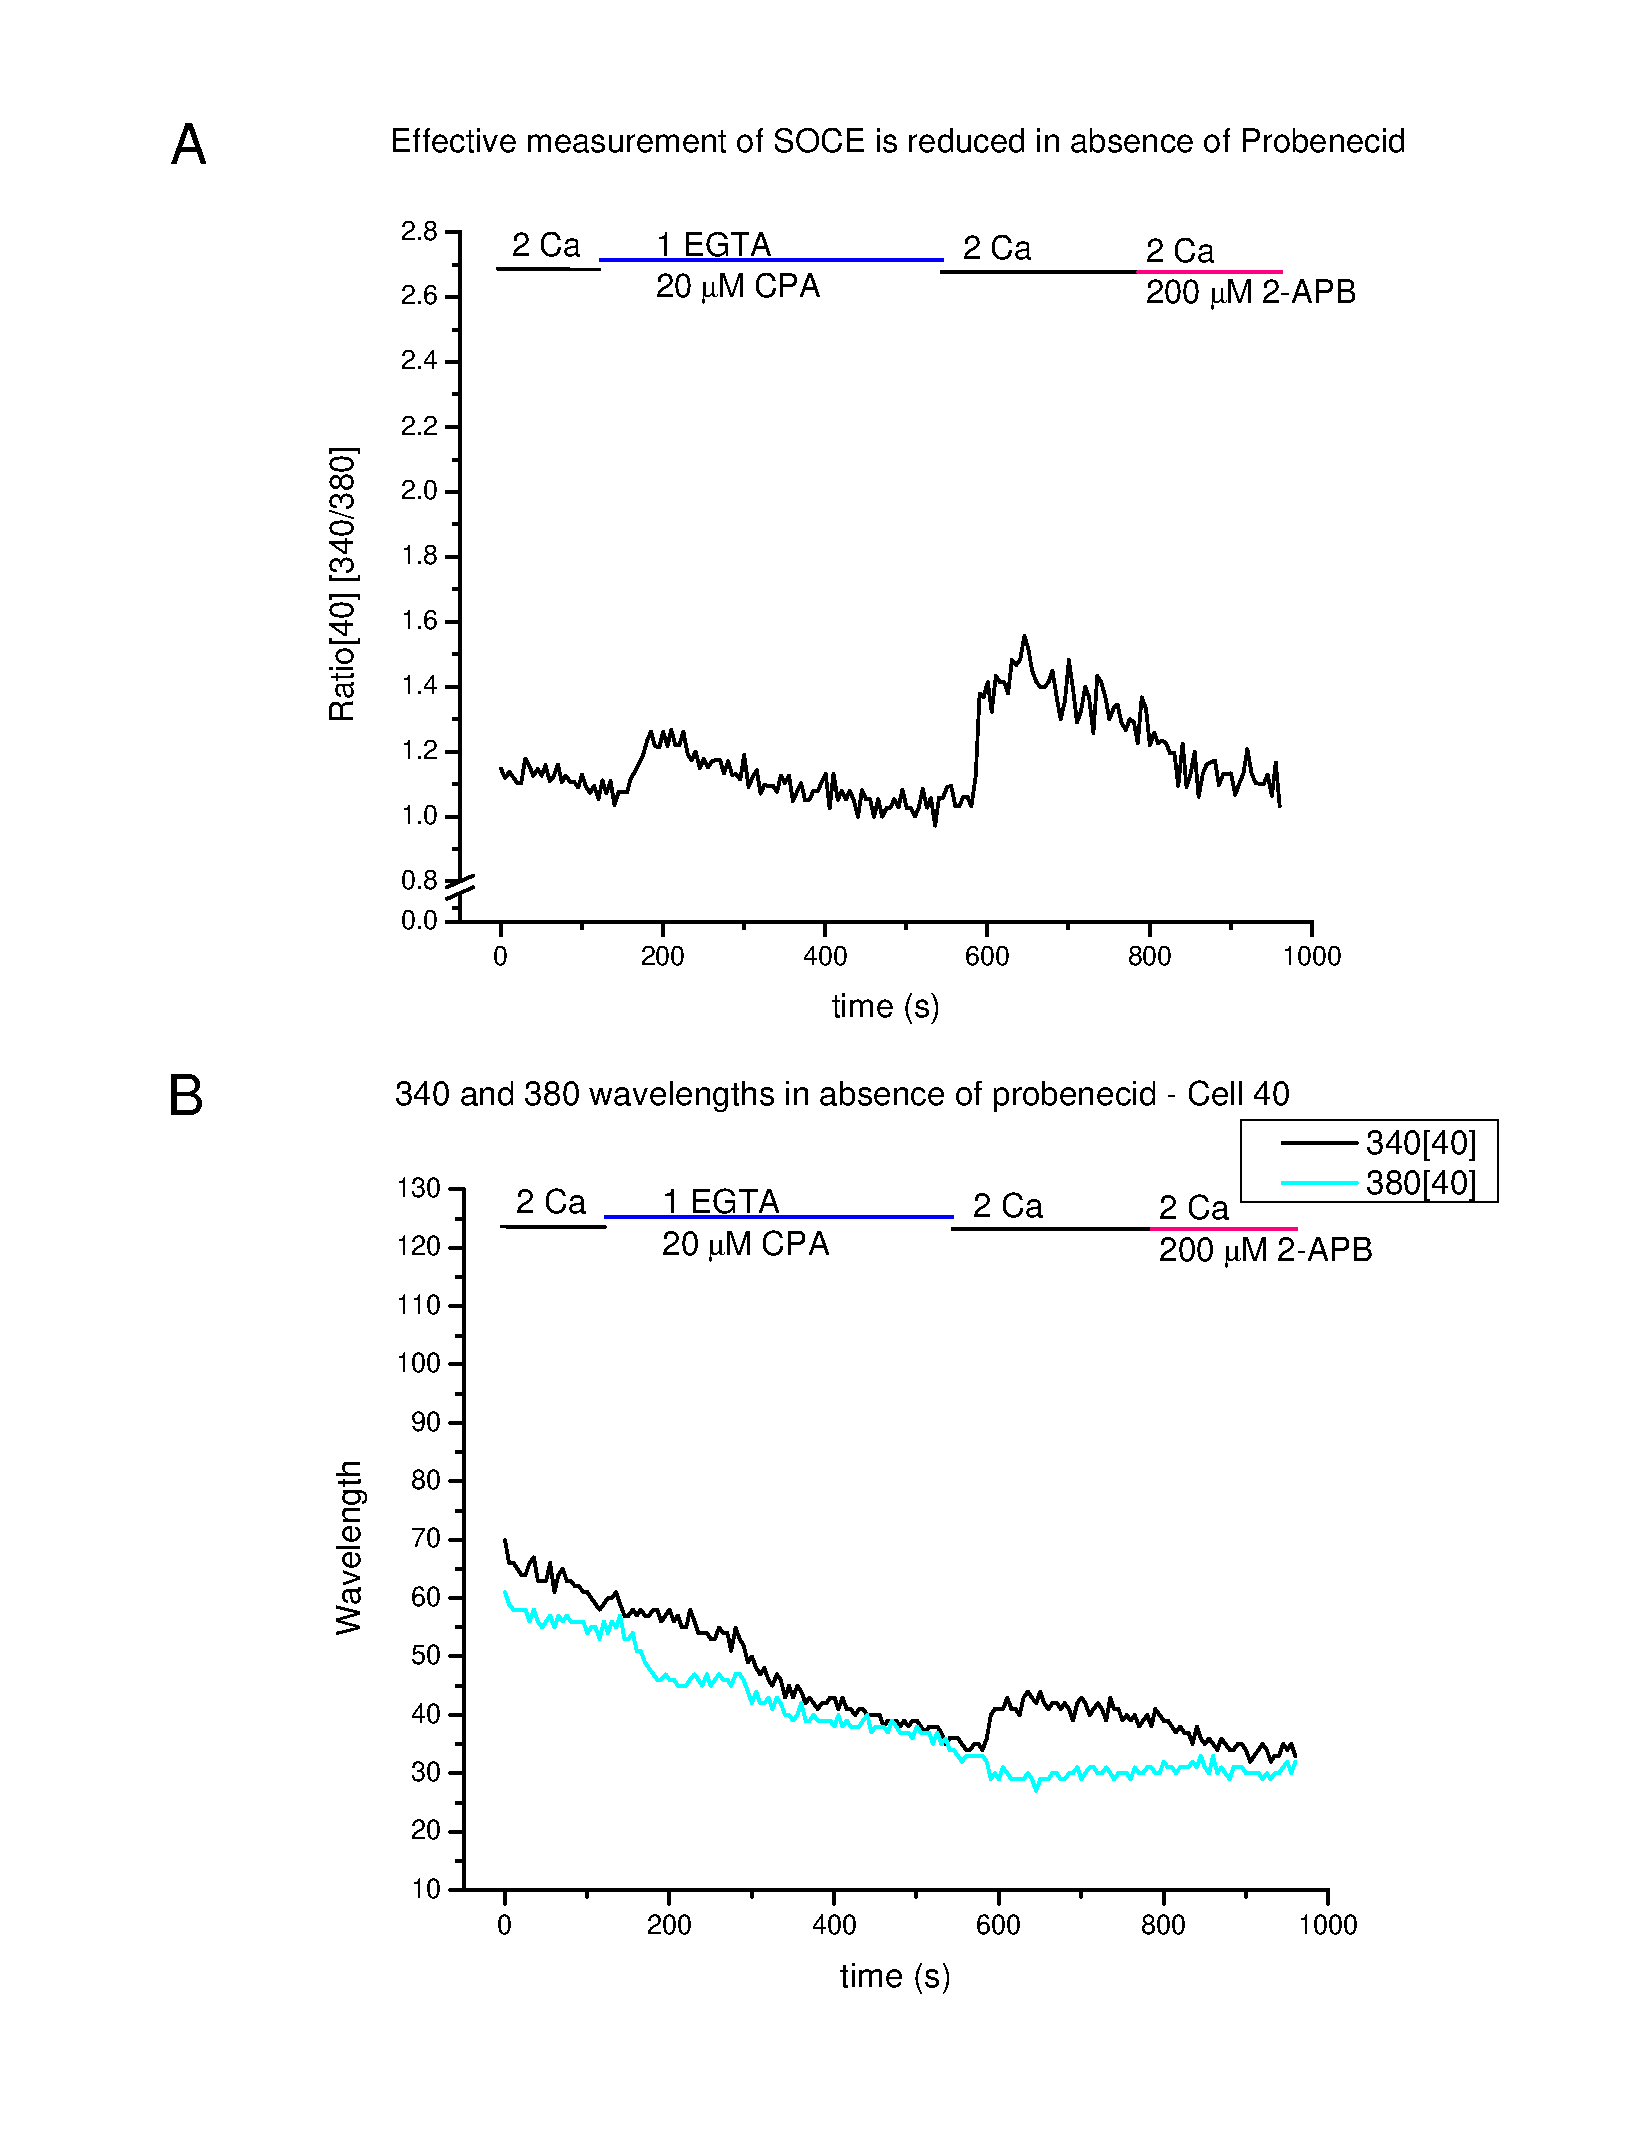
\includegraphics[scale=0.5]{Figures/s2_cell40_nopro.pdf}
\caption[Absence of probenecid gives less efficient dye loading in S2 cells]
	{{\bfseries The absence of probenecid results in less efficient dye loading in S2 cells}. ({\bfseries A}) The ratio of the 340 nm and 380 nm wavelengths of an individual cell during the course of one perfusion experiment where probenecid was omitted from the incubation solution. ({\bfseries B}) The individual 340 nm and 380 nm wavelength values, which produced the ratio seen in {\bfseries A}.}
\label{fig:s2_no_pro}
%\end{center}
\end{figure}

Figure~\ref{fig:s2_no_pro}A shows a recording from an individual S2 cell loaded without probenecid being present in the dye-loading solution (DLS).  Figure~\ref{fig:s2_no_pro}B shows the individual 340 and 380 nm wavelength values that produced the trace in A. Though the trace of the ratio hides it, we see that both wavelengths values start decreasing immediately after the start of the experiment. The decreasing values continue to the end of the experiment. The decay likely reflects leakage of Fura-2 which takes place in S2 cells if probenecid is absent in the DLS \citep{DiVirgilio1990}. The \Ca{} ratios reported after SOCE, upon reintroduction of 2 Ca are  also shown to be low here. This is most likely an artifact caused by less Fura-2 availability, thereby limiting the amount of cytoplasmic \Ca{} that can be measured.

\newpage

\begin{figure}[!ht]
%\begin{center}
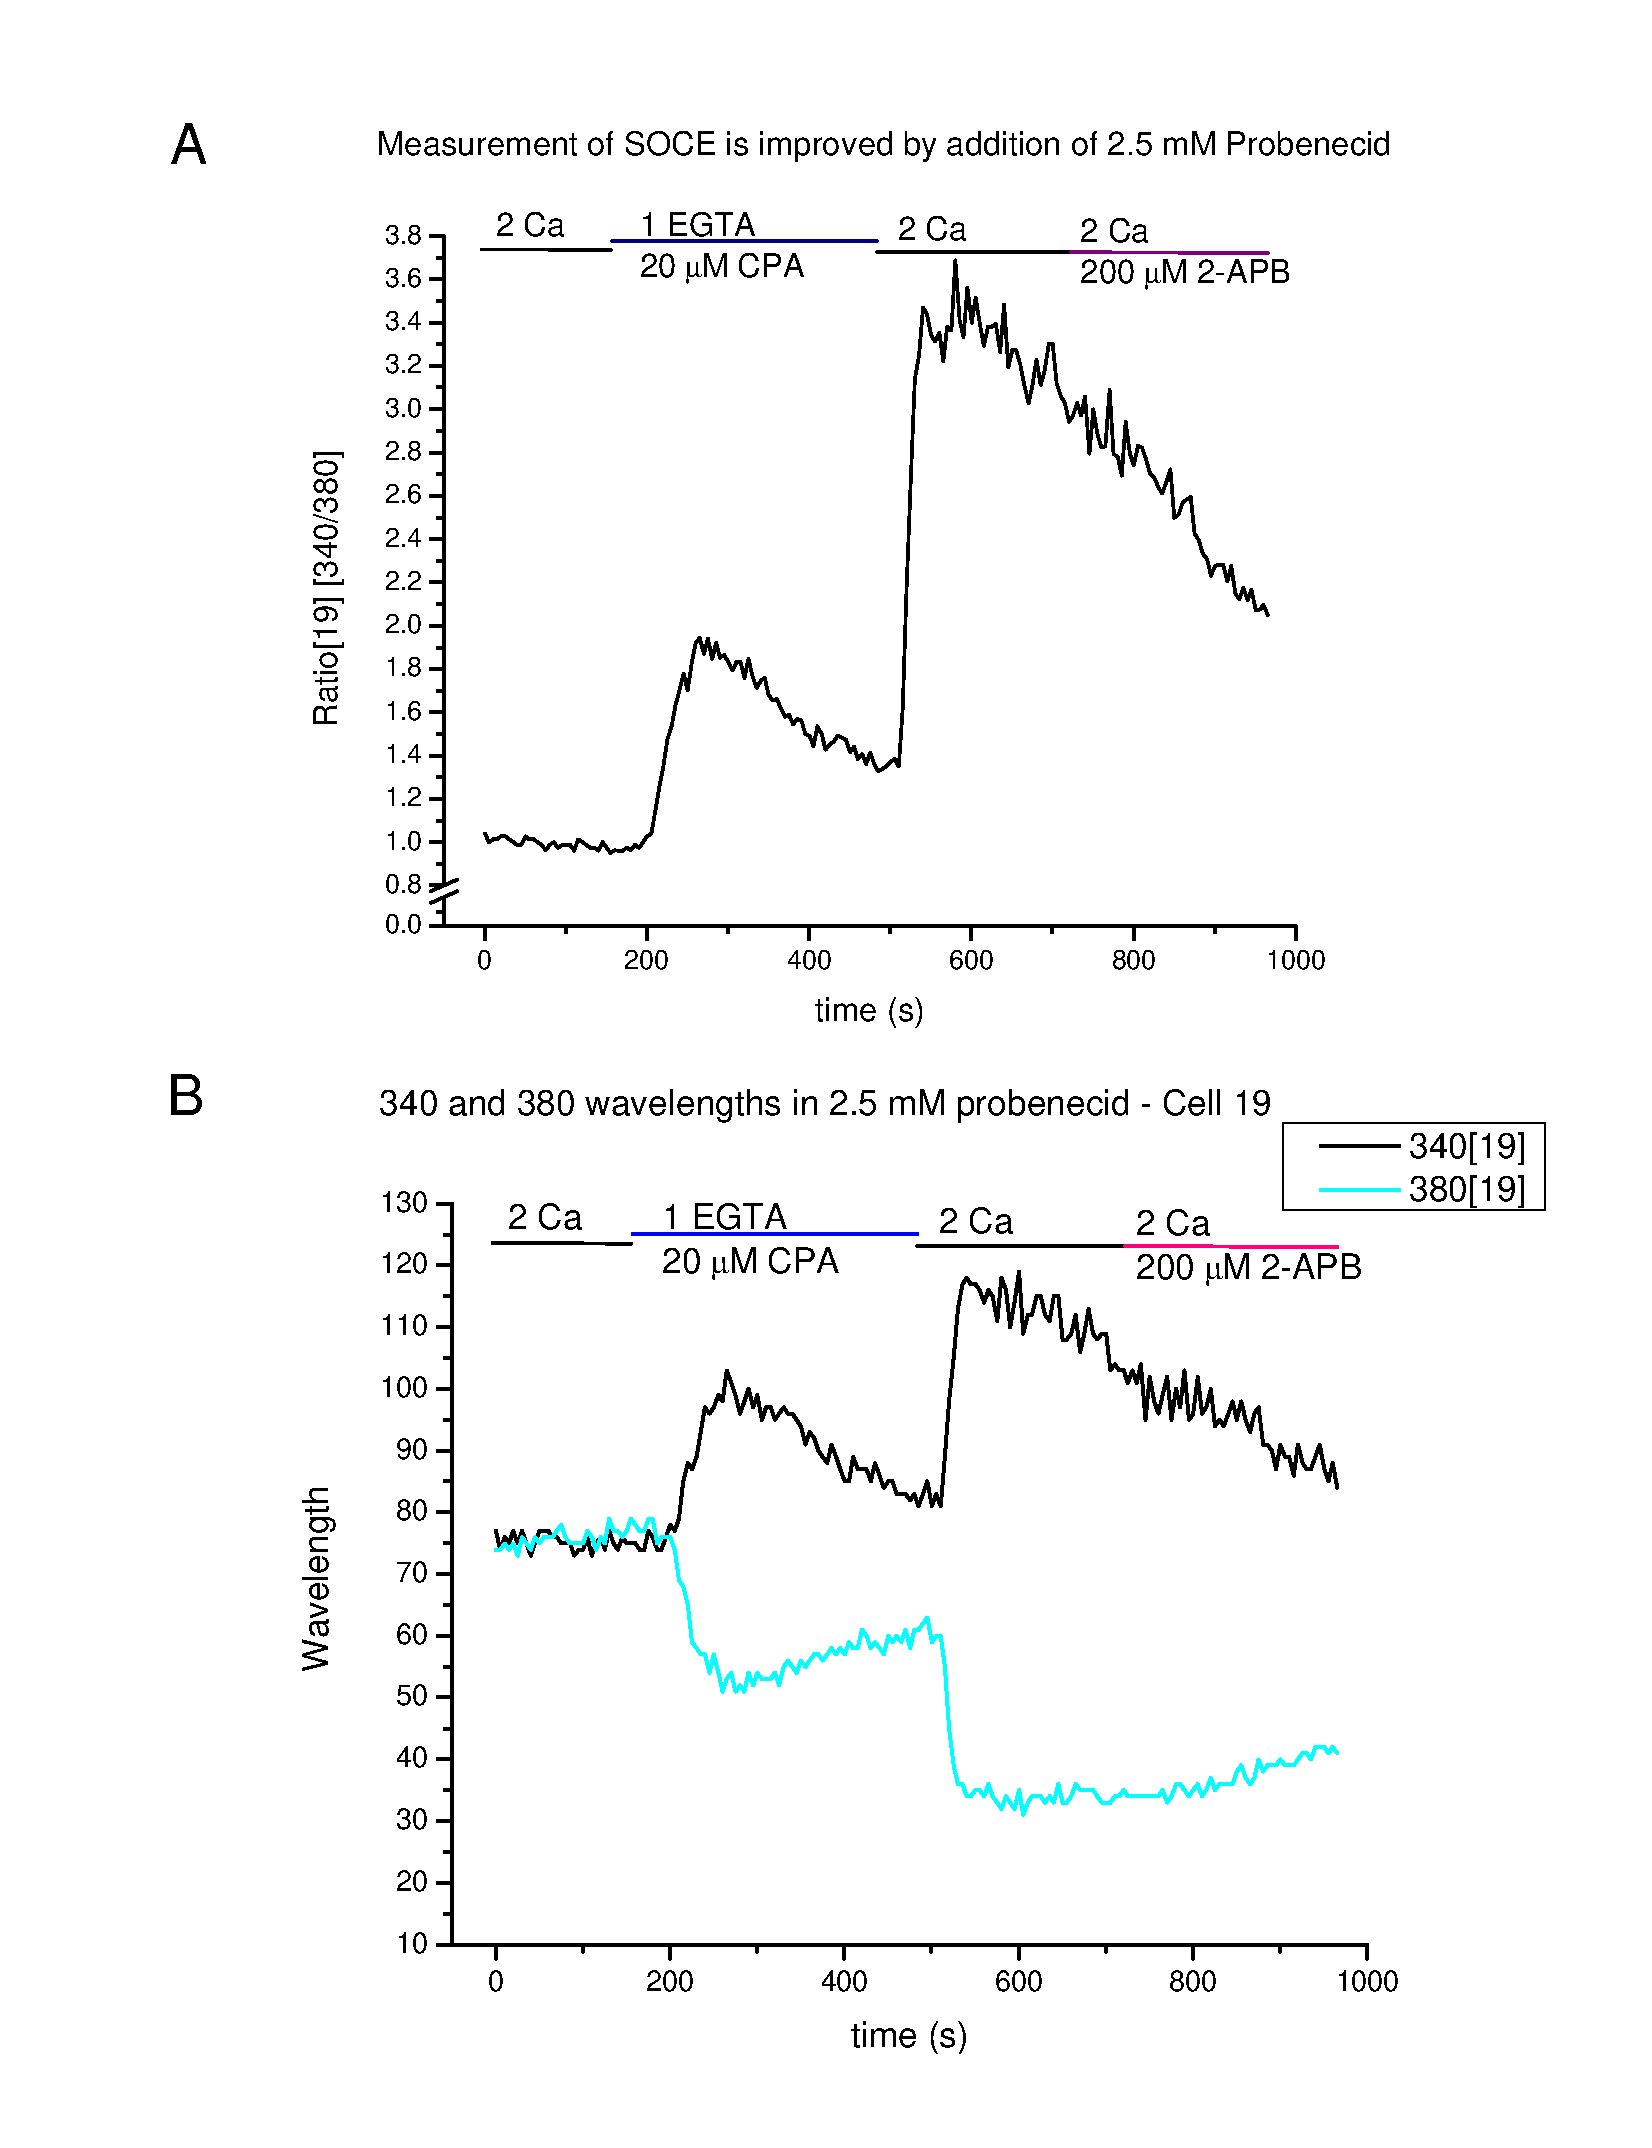
\includegraphics[scale=0.52]{Figures/s2_cell19_pro.pdf}
\caption[Probenecid improves dye loading in S2 cells]
	{{\bfseries The presence of 2.5 mM probenecid improves dye loading in S2 cells}. ({\bfseries A}) The ratio of the 340 nm and 380 nm wavelengths of an individual cell during the course of a perfusion experiment where 2.5 mM probenecid was included in the incubation solution. ({\bfseries B}) The individual 340 nm and 380 nm wavelength values, which produced the ratio seen in {\bfseries A}.}
\label{fig:s2_with_pro}
%\end{center}
\end{figure}

Figure~\ref{fig:s2_with_pro}A shows a sample recording from a cell incubated with DLS containing 2.5 mM probenecid. The ratio is robust and provides better resolution than the trace in figure~\ref{fig:s2_no_pro}. Figure~\ref{fig:s2_with_pro}B gives the individual 340 nm and 380 nm wavelengths which were used to obtain the ratio in A. We are able to clearly see the reciprocal nature of the 340 nm and 380 nm wavelength values. The steady decline of the values over the course of the experiment is no longer apparent. Probenecid has stopped or greatly slowed leakage of Fura-2 from the cytosol. As a result, we are able to record higher \Ca{} transients as more Fura-2 is available as the experiment proceeds, compared to cells loaded without probenecid. This is readily apparent in the SOCE portion of the trace. 

\newpage

\begin{figure}[!ht]
\centering
\subfloat{
	\begin{lpic}[clean]{Figures/no_pro(0.8)}
	%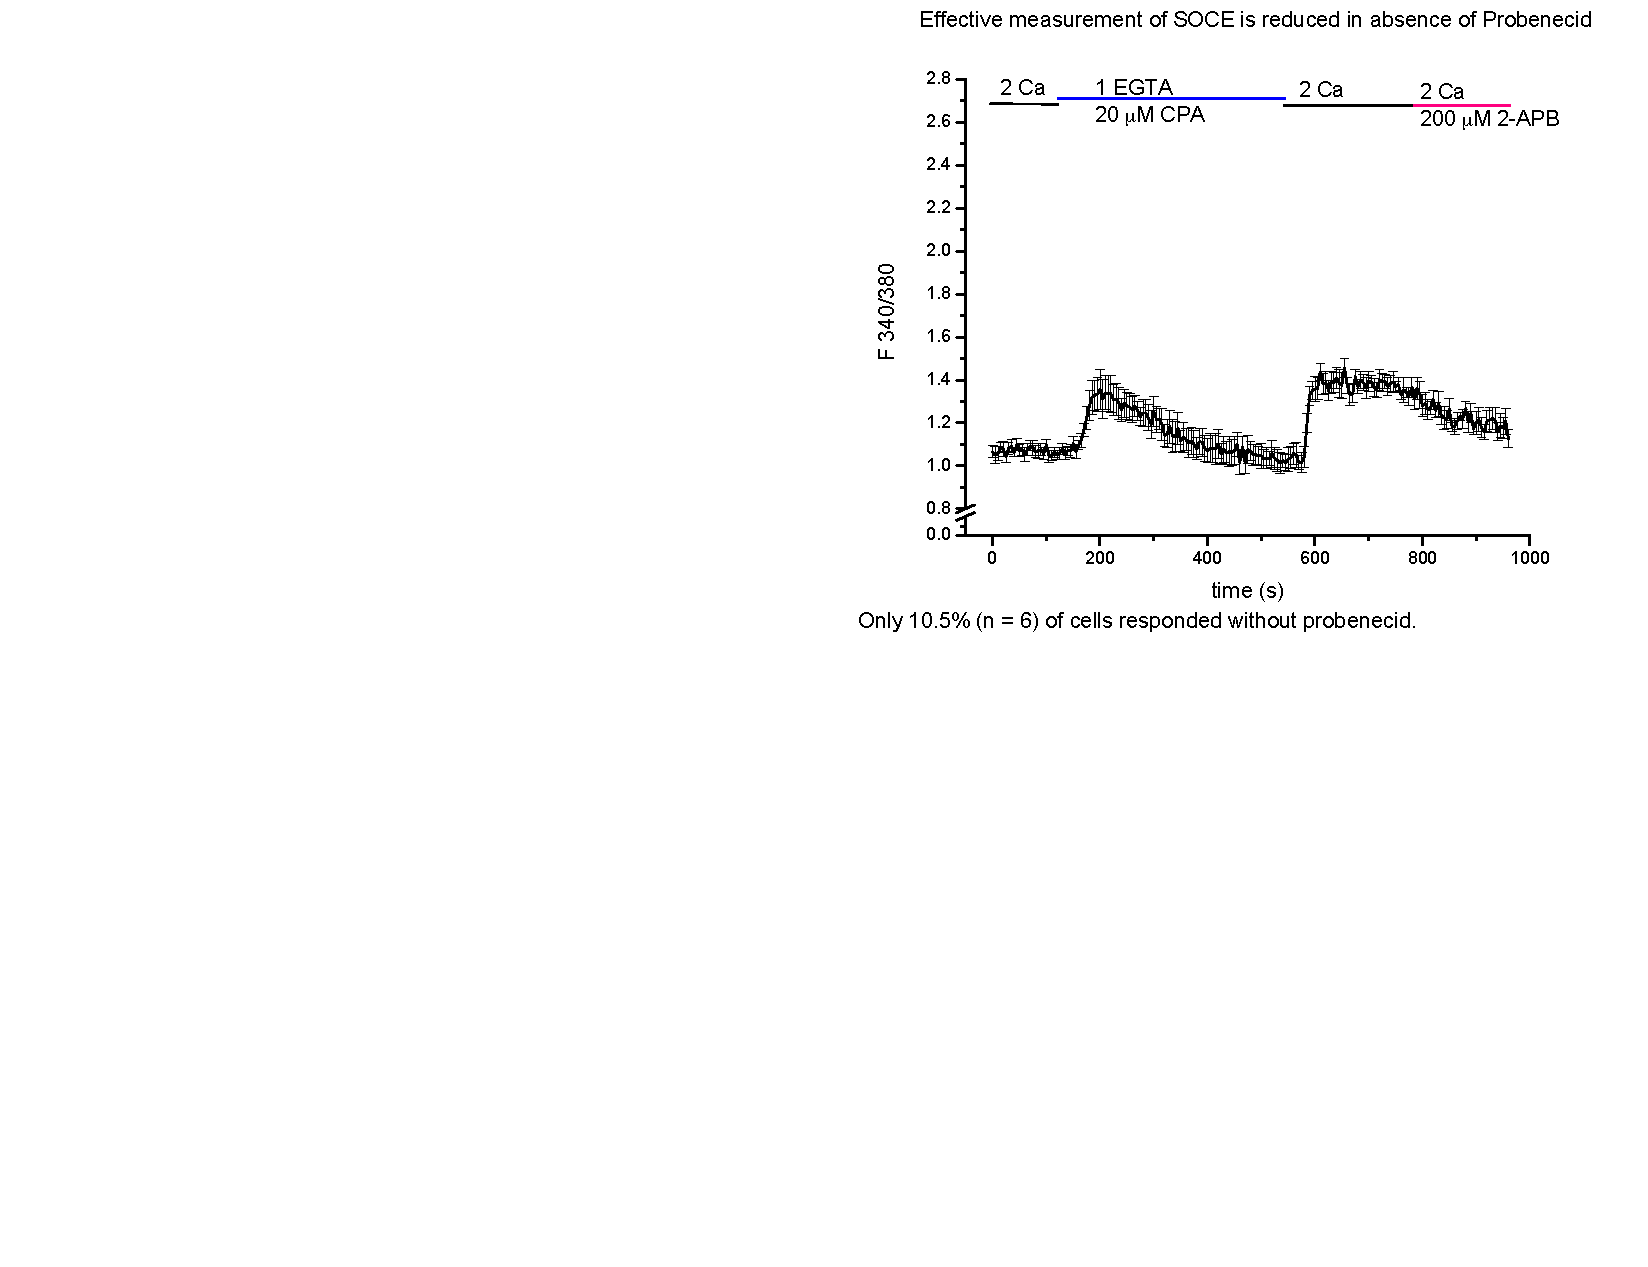
\includegraphics[scale=0.9]{Figures/no_pro} 
		\lbl[bl]{1,105; \bfseries A}
	\end{lpic}
}
	
\subfloat{
	\begin{lpic}[clean]{Figures/with_pro(1.3)}
	%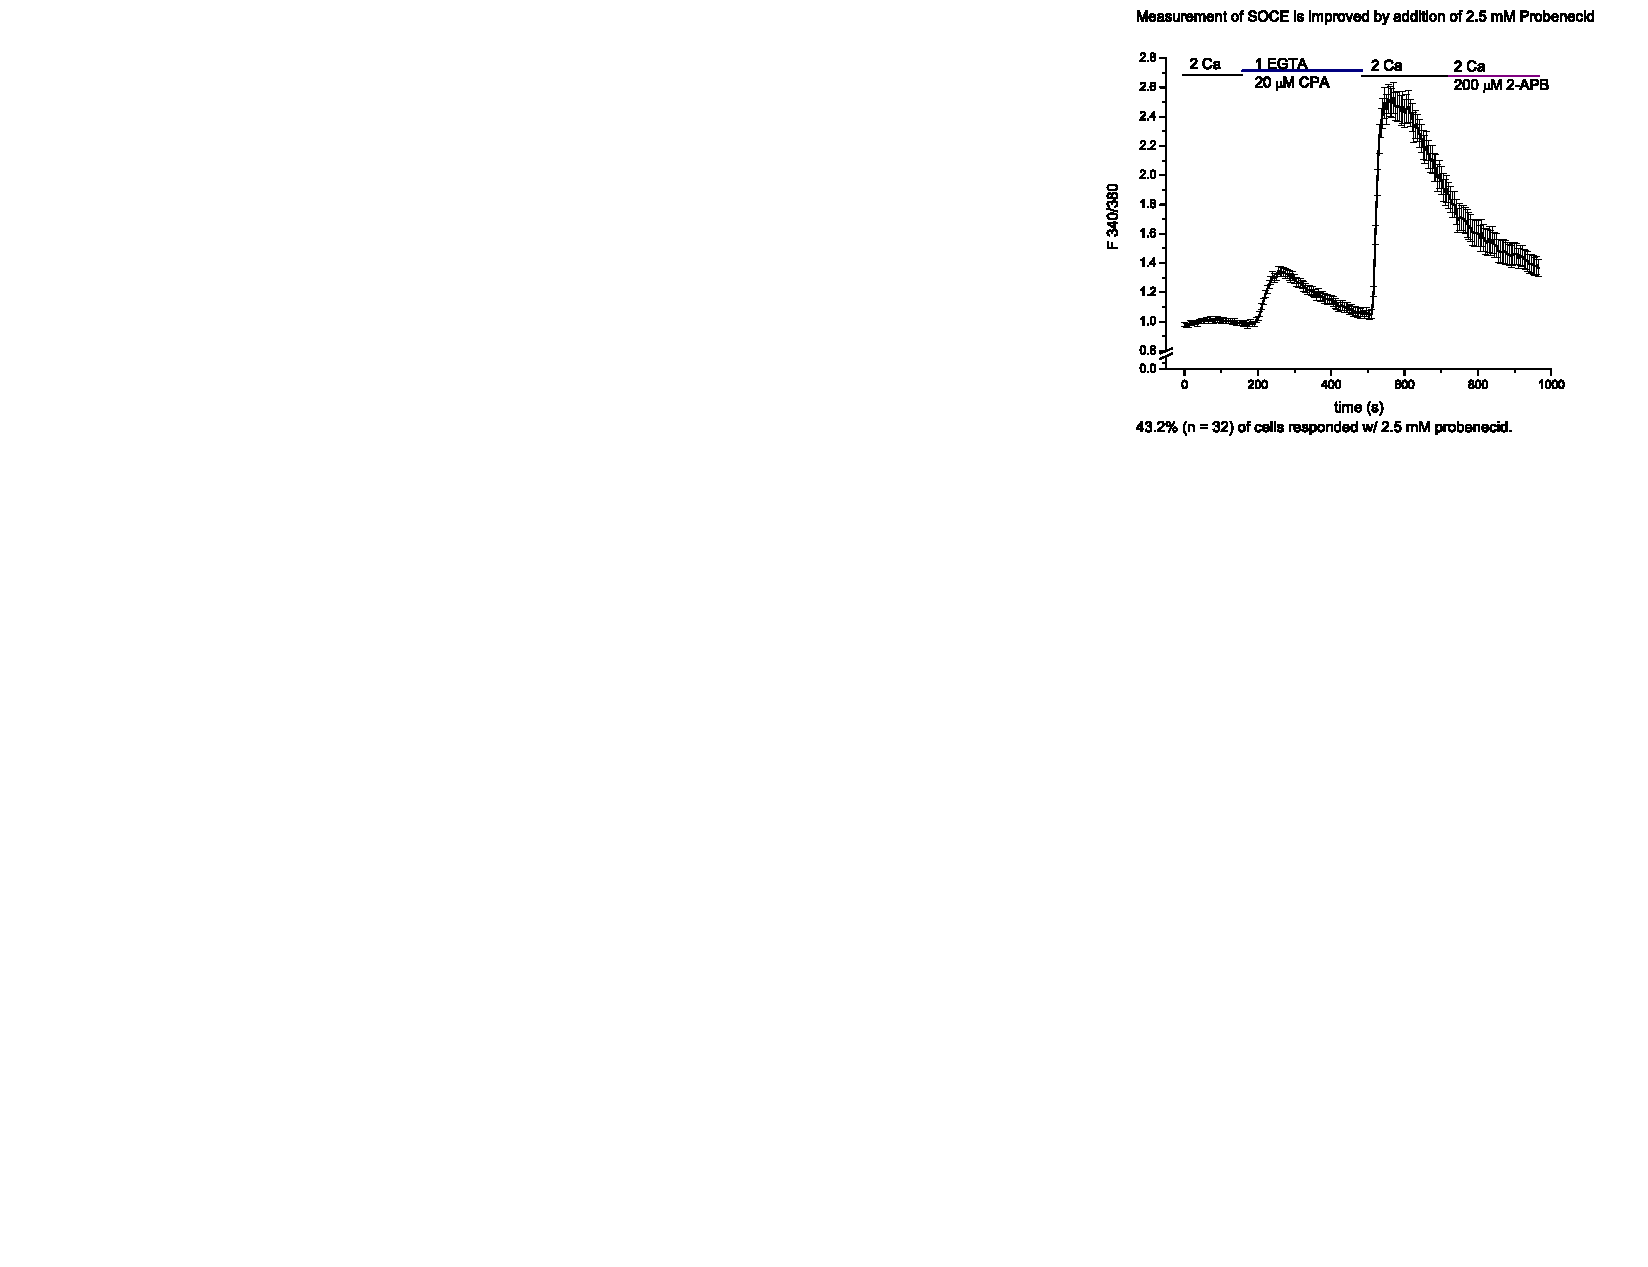
\includegraphics[scale=1.3]{Figures/with_pro}
		\lbl[bl]{6,76; \bfseries B}
	\end{lpic}
}
\caption[Addition of Probenecid improves \Ca{} recordings]{{\bfseries Addition of Probenecid improves \Ca{} recordings}. 
({\bfseries A}) Recordings taken from a population of cells incubated in dye-loading solution that did not contain probenecid ({\bfseries B}) Recordings taken from a population of cells incubated in dye-loading solution that contained 2.5 mM probenecid.}
\label{fig:s2_pro_compare}
\end{figure}

Figure~\ref{fig:s2_pro_compare} shows a population of cells loaded without (A) and with (B) probenecid. We are able to observe a larger \Ca{} transient, due to more Fura-2 being available. Also, addition of probenecid results in more cells meeting the selection criteria for data collection. This can be attributed to Fura-2 retention in probenecid-treated S2 cells. The result is more dye being available at the start of the experiment, and as it progresses. 

Unhealthy cells, cells with damaged plasma membranes may also be omitted from the data set in a reliable, unbiased manner after probenecid treatment. Such cells would still display characteristics of untreated cells such as pronounced, persistent dye leakage.

Conditions for selecting data were formulated after examining individual 340 nm and 380 nm wavelength traces for probenecid-treated and untreated cells. Three out of six cells in A, had either 340 nm or 380 nm wavelength values below 40. This led us to use 40 as a cutoff value for data selection. For the S2 cells selected, both the 340 nm and 380 nm wavelength values stayed at or above 40 during the initial 2 Ca perfusion. This allowed for elimination of cells which were poorly loaded with Fura dye.
%leaky, even after treatment with probenecid  which, for reasons explained above, were deemed undesirable.

%\begin{figure}[htbp]
%\begin{center}
%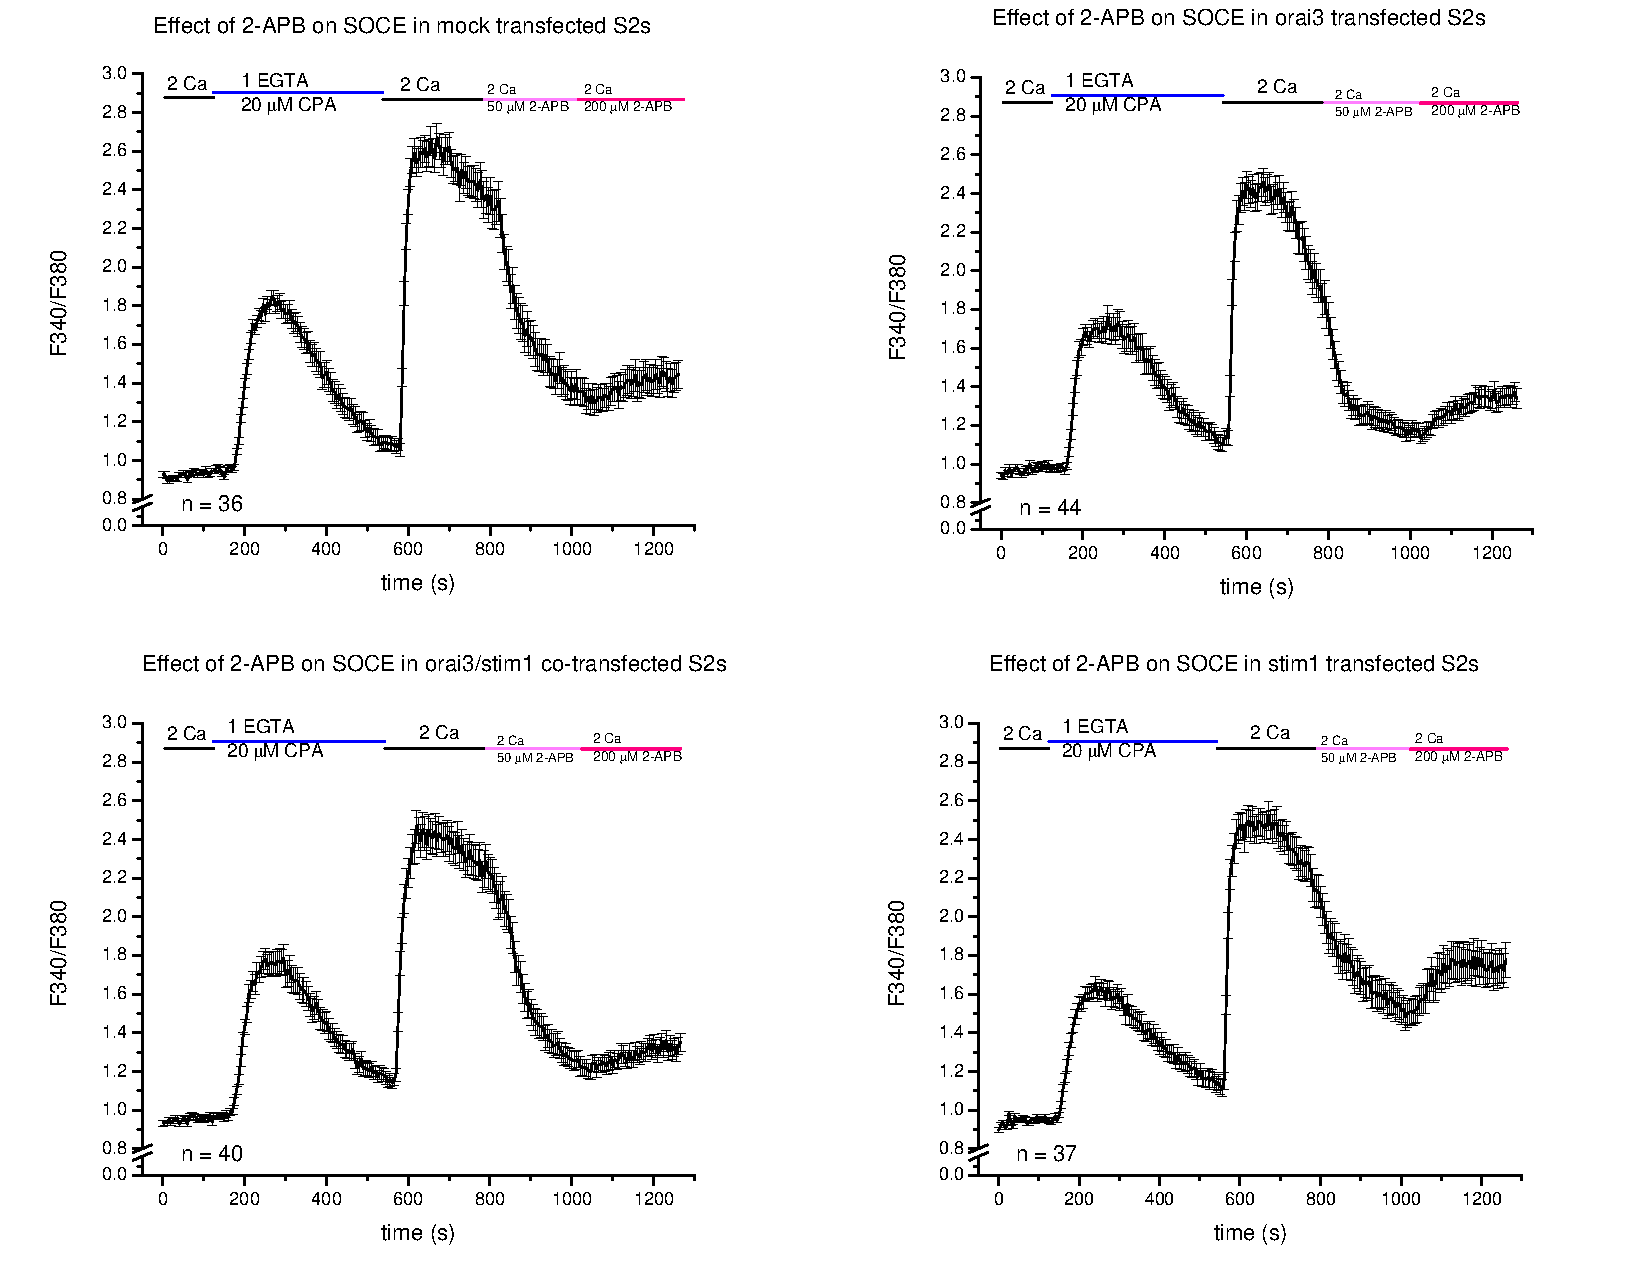
\includegraphics[clip=true, scale=0.61, trim=8mm 0 10mm 0]{Figures/s2_sample_composite}
%\caption{Ca$^{2+}$ measurements in transfected S2 cells perfused with 2-APB}
%\label{fig:s2_composite}
%\end{center}
%\end{figure}
\newpage

\begin{figure}[!ht]
	\centering
	\subfloat{
		\begin{lpic}[clean]{Figures/s2_ca_mock5_all(0.45)}
		%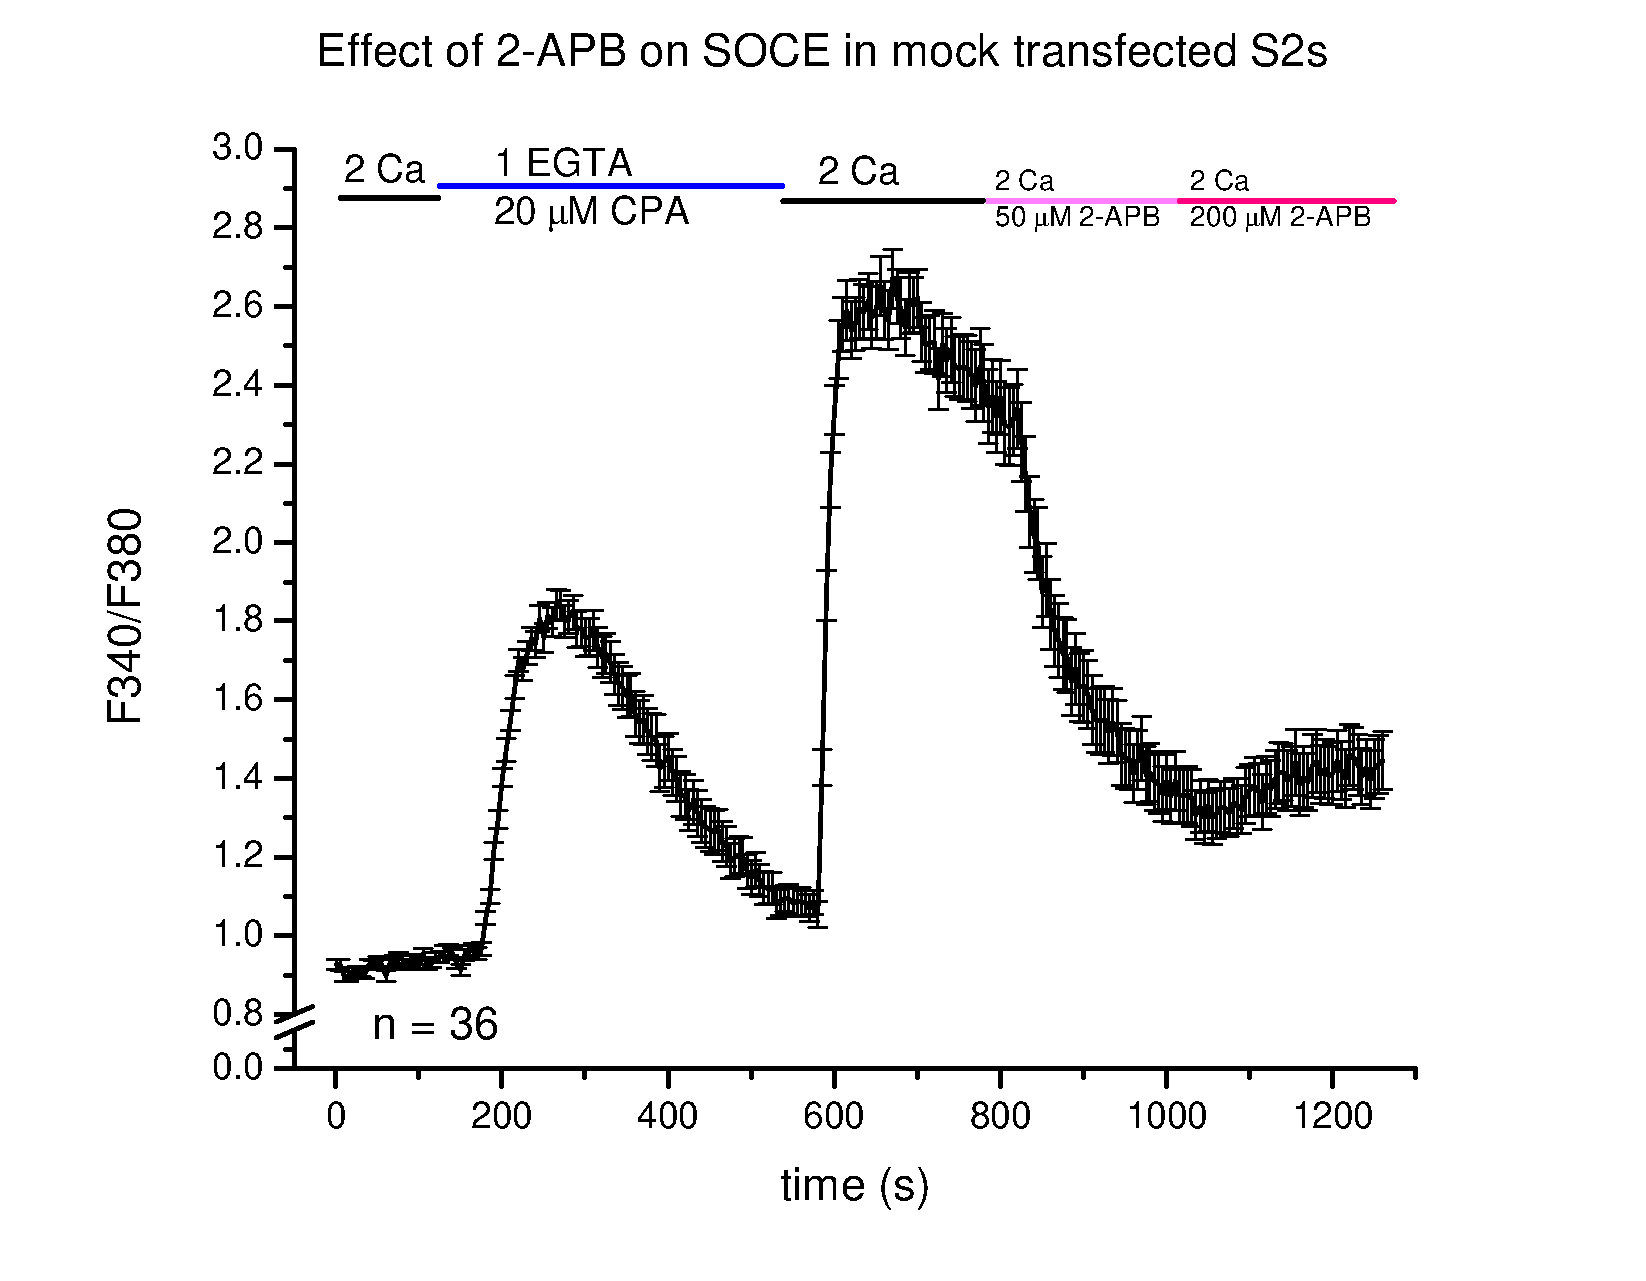
\includegraphics[scale=0.5]{Figures/s2_ca_mock5_all.pdf}
		\lbl[bl]{5,205; \bfseries A}
		\end{lpic}
	}
	
	\subfloat{
		\begin{lpic}[clean]{Figures/s2_ca_orai3_all5(0.45)}
		%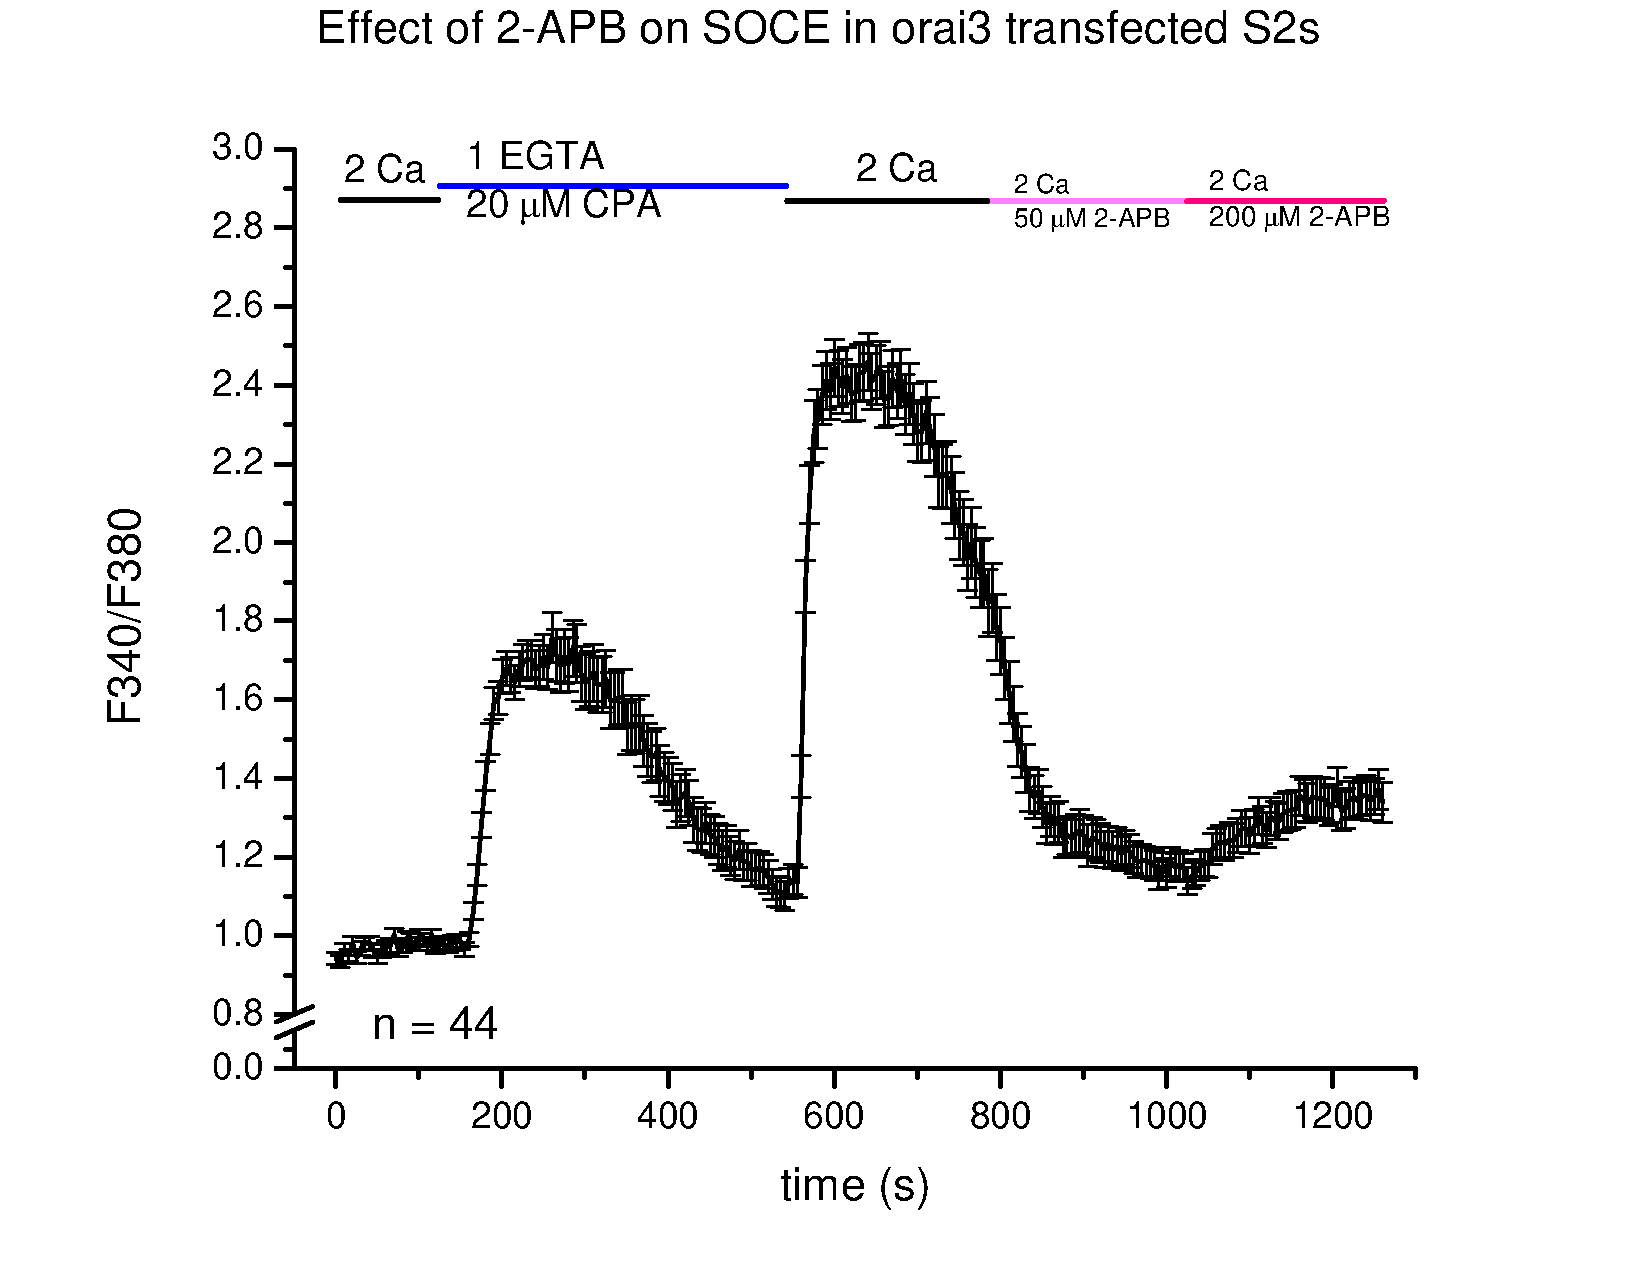
\includegraphics[scale=0.5]{Figures/s2_ca_orai3_all5.pdf}}
			\lbl[bl]{5,210; \bfseries B}
		\end{lpic}
	} 
	\caption[\Ca{} measurements in transfected S2 cells perfused with 2-APB]{{\bfseries \Ca{} measurements in transfected S2 cells perfused with 2-APB}. 	
	The lines above the trace are labeled with the solutions perfused during those times. \textbf{A}) A trace of mock-transfected S2s showing the effect of 2-APB on SOCE. \textbf{B}) A trace of Orai3-transfected S2s showing the effect of 2-APB on SOCE.}
	\label{fig:s2_composite}
\end{figure}
	
\begin{figure}[!ht]
	\centering
	\ContinuedFloat
	\subfloat{
		\begin{lpic}[clean]{Figures/s2_5_o3s1_all(0.42)}
		%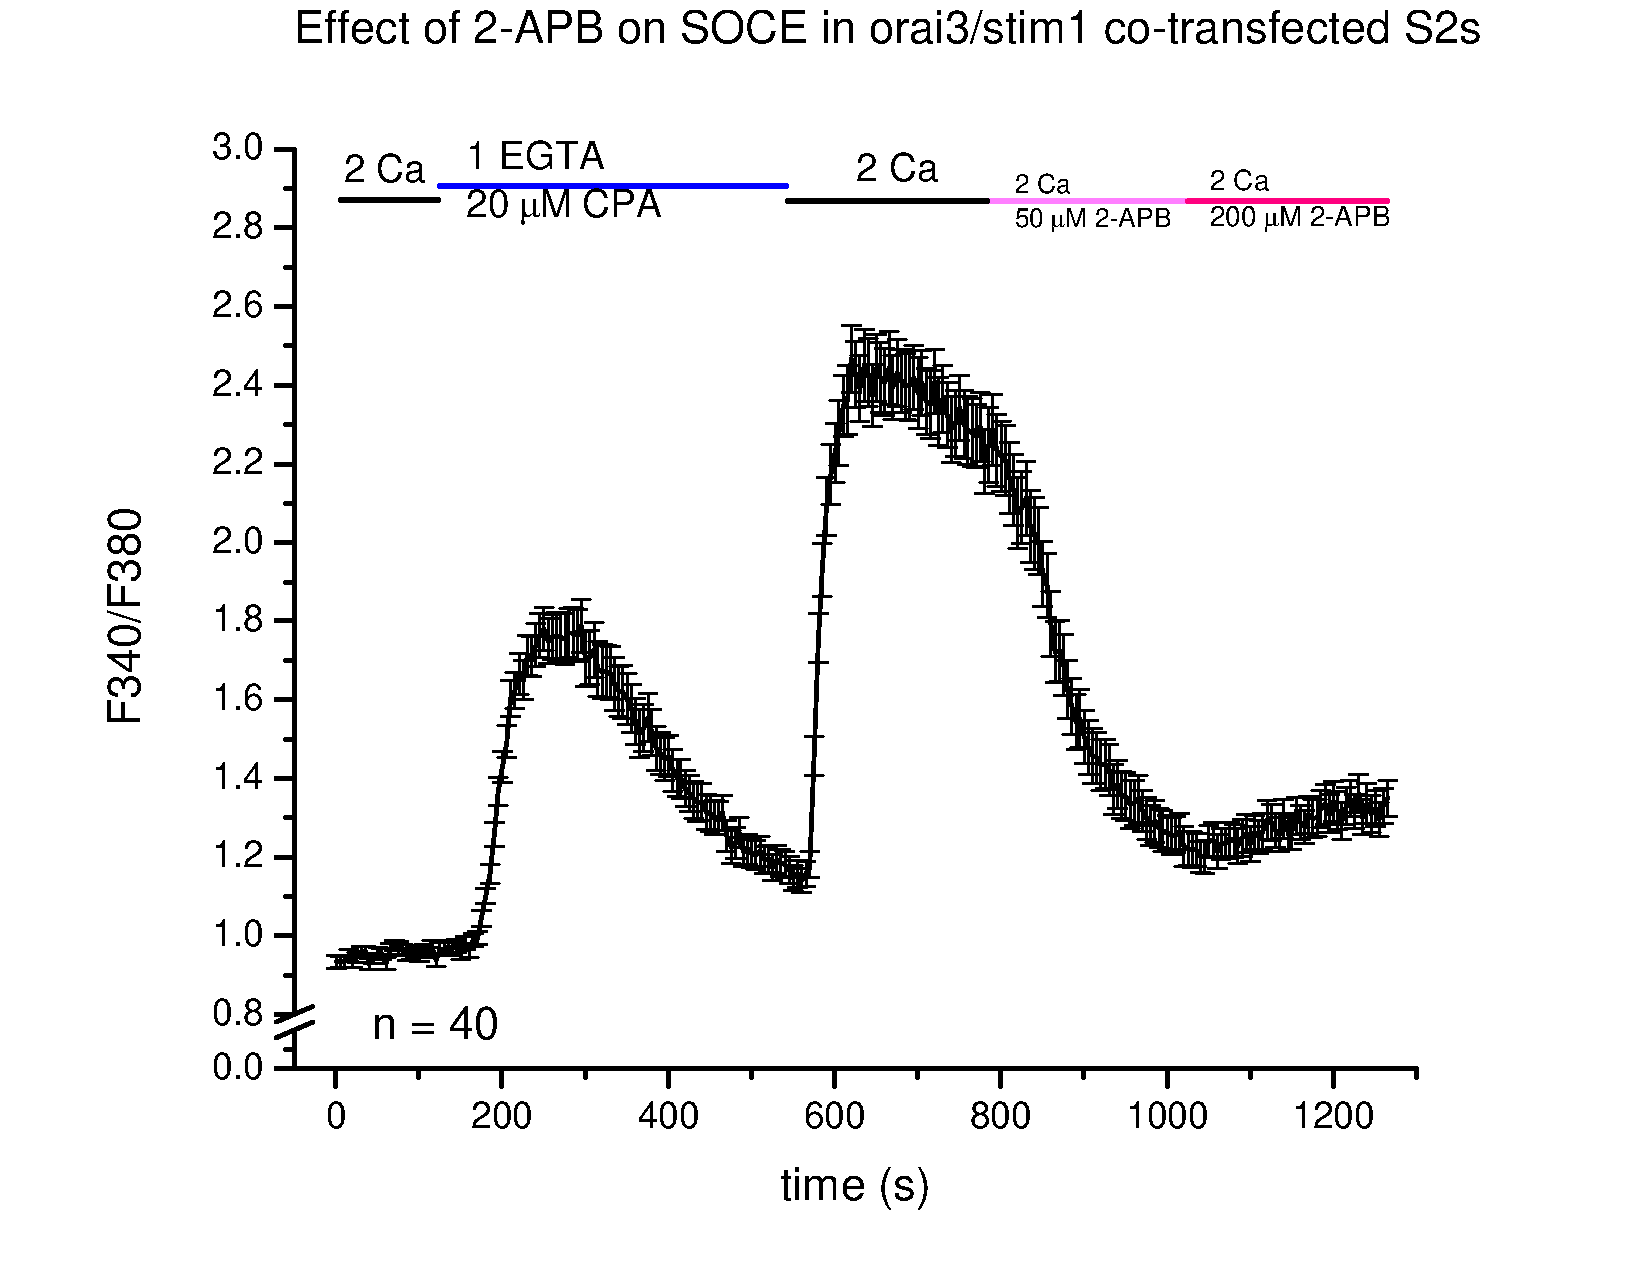
\includegraphics[scale=0.5]{Figures/s2_5_o3s1_all.pdf}
			\lbl[bl]{5,210; \bfseries C}
		\end{lpic}
	}
	
	\subfloat{
		\begin{lpic}[clean]{Figures/s2_ca_stim1_3_all(0.42)}
		%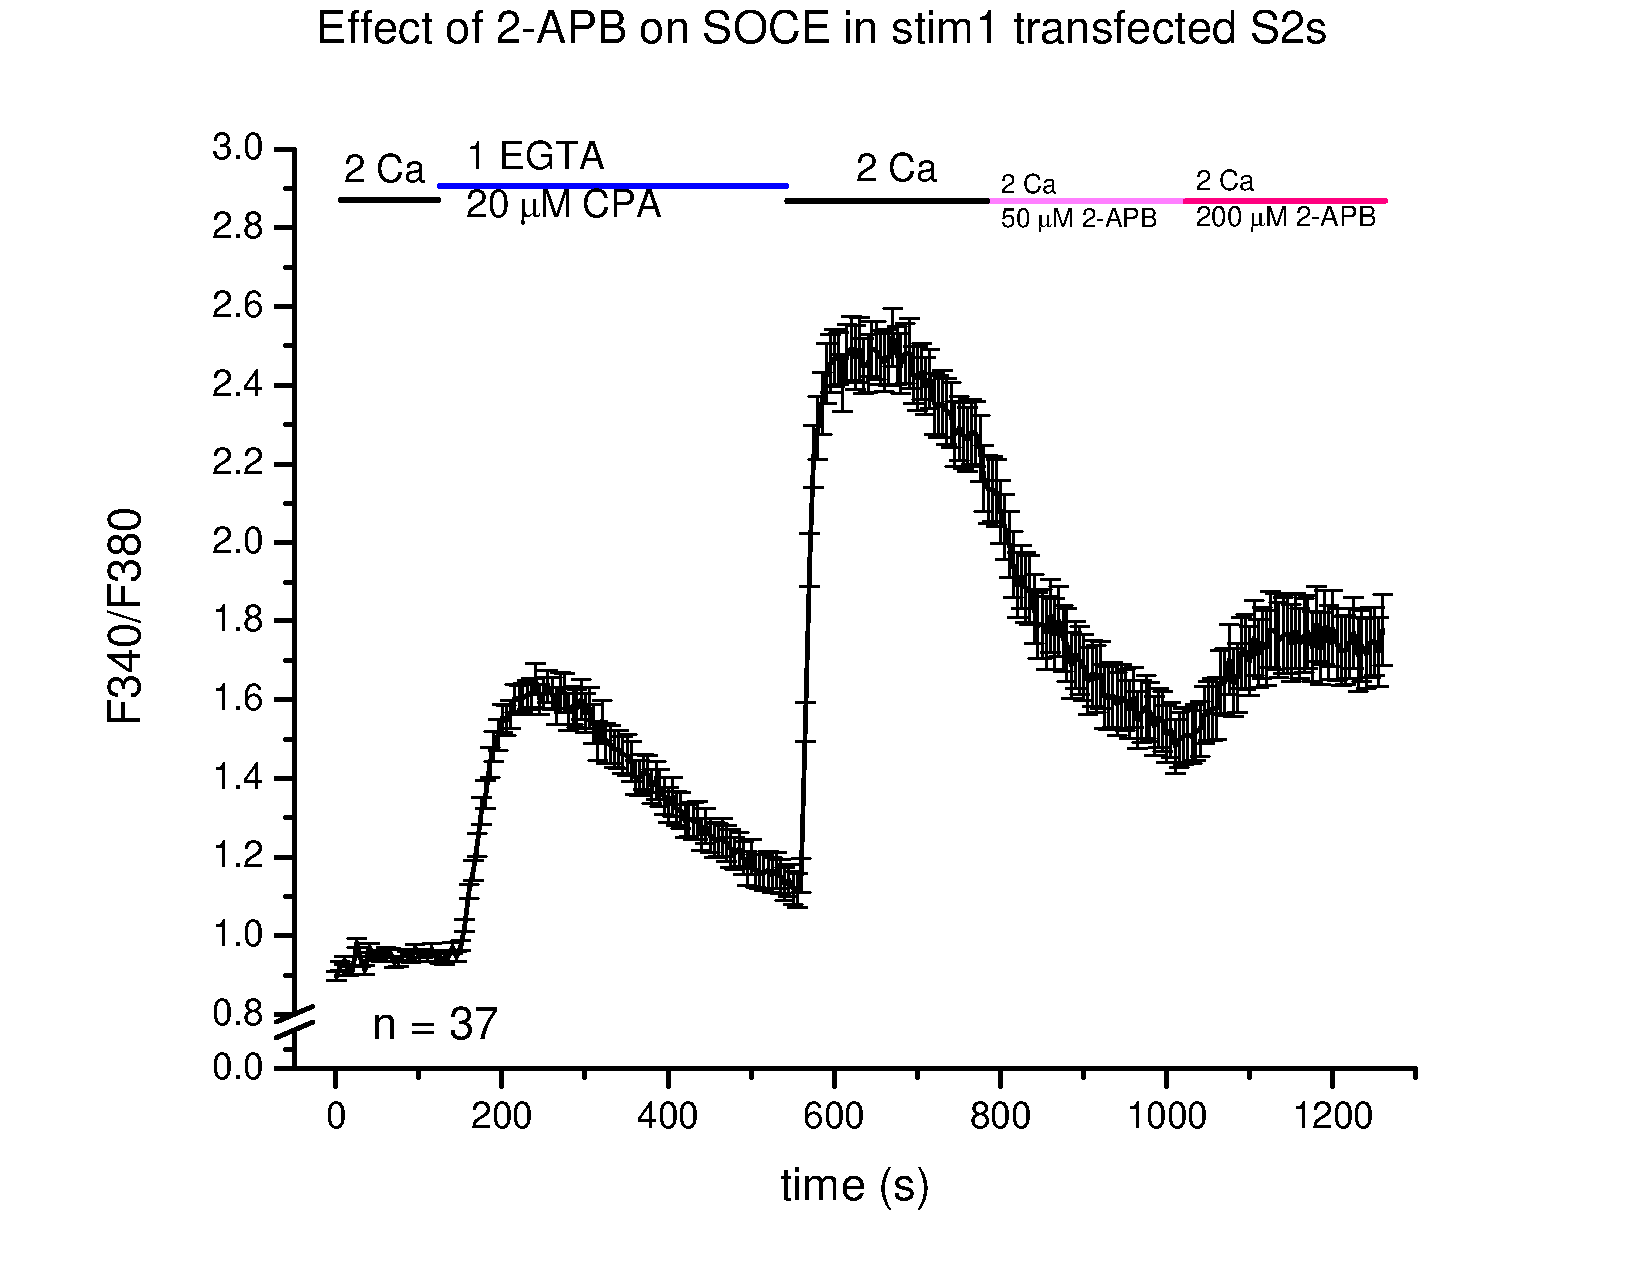
\includegraphics[scale=0.5]{Figures/s2_ca_stim1_3_all.pdf}
			\lbl[bl]{5,210; \bfseries D}
		\end{lpic}
	}
	\caption[]{{\bfseries Ca$^{2+}$ measurements in transfected S2 cells perfused with 2-APB}. 	
	The lines above the trace are labeled with the solutions perfused during those times. \textbf{C}) Sample trace of Orai3+\stim{}-transfected S2s showing the effect of 2-APB on SOCE. \textbf{D}) Sample trace of \stim{}-transfected S2s showing the effect of 2-APB on SOCE.}
	\label{fig:s2_composite}
\end{figure}


The composite in Figure~\ref{fig:s2_composite} shows representative traces for \Ca{} imaging experiments where S2 cells have been mock-transfected or transfected with Orai3, \stim{}, or Orai3+\stim.
In Figure~\ref{fig:s2_composite}A we see an average of several traces giving the result of an experiment done on mock-transfected S2s. Initially, the 2 Ca response of these mock-transfected S2s is relatively stable. Upon introduction of 20 $\mu$M CPA in 1 EGTA, we observe an increase in the F340/F380 ratio. This indicates an increase in cytosolic free \Ca, resulting from leakage of \Ca{} from the ER. This \Ca{} leak achieves a maximum and subsequently declines. The decline phase is indicative of \Ca{} being pumped out of the cell, shuttled to non-ER compartments, such as the mitochondria, or being bound by cytosolic \Ca{} chelators. Transport of \Ca{} to the ER is prevented by CPA, which blocks the SERCA pump. 

After $\sim$7 minutes of perfusion in 1 EGTA/20 $\mu$M CPA, \Ca{} is reintroduced. The mock-transfected S2s then exhibit SOCE, and a second \Ca{} transient forms at this stage. The maximal \Ca{} entry after 2 Ca reintroduction is greater than maximal \Ca{} release from the ER.  \dorai{} channels responsible for SOCE in S2 cells are able to open quickly, allowing \Ca{} into the cell shortly after switching to the 2 Ca solution.
We eventually begin to see less \Ca, which can be attributed to \dorai{} channels closing, slowing \Ca{} entry.

After 4 minutes in 2 Ca, 50 $\mu$M 2-APB is added to the perfusion solution. We see for the mock-transfected S2 cells, that the gradual decline in \Ca{} becomes sharper, shortly after addition of 2-APB. This is expected because at these concentrations 2-APB is inhibitory for \dorai{} \citep{Yeromin:2004p520}. The decline in \Ca{} continues during the 4 minutes in 50 $\mu$M 2-APB. 

After 4 minutes in 2 Ca with 50 $\mu$M 2-APB, the 2-APB concentration is increased to 200 $\mu$M 2-APB. This solution was perfused across the cells for another 4 minutes and then the experiment was stopped. During this time we observe what seems to be a slight increase. The overlap of the error bars along the trace indicate that, while there is a trend toward an increase, further analysis is required to determine its significance. In order to address the question of what happens to \Ca{}, the area under the curve was calculated for each 4-minute section after store-depletion occurred for each group of transfected cells. 

Figure~\ref{fig:s2_composite}B shows an average trace of an experiment performed on Orai3-transfected S2 cells. The initial and store-depletion phases are similar to those in the mock-transfected S2s. 2 Ca reintroduction shows a swift onset of SOCE. The expected increase in \Ca{} after addition of 50 $\mu$M 2-APB was not seen, however. Addition of 200 $\mu$M 2-APB seemed to result in a marginal increase in \Ca{} entry. The \Ca{} content of this 200 $\mu$M 2-APB phase was analyzed further and no significant change from the mock was found (see Figure~\ref{fig:s2_2apb_bar}).

%Discussion: There are a few possibilities for why this happened. The most obvious is that while Orai3 RNA production was induced with \cuso, actual protein production did not occur.Another possibility is that the transfection efficiency was consistently low with the TransIT-2020 reagent and Orai3 vector DNA. This may have resulted in poor expression of Orai3 and a paucity of Orai3 protein translation, leading to a deficiency in Orai3 channels expressed at the cellular surface. Another possibility is that, because of how closely related Orai3 and \dorai{} are, Orai3 forms heterodimers with \dorai, and adopts a phenotype primarily \dorai{} in nature.
%Testing protein expression of Orai3 proteins is possible, by isolating proteins from cells and performing a Western Blot using antibodies purchased to Orai3. 
%The generation of stable cell lines expressing Orai3 will facilitate experiments important for testing the other possibilities. \rnai{} knockdown of native \dorai{} will enable these experiments to be carried out in a background free of Orai which may be interfering with our heterologous Orai3 channel assembly. 

Since no distinct effect of 2-APB was observed in S2s transfected with Orai3 only, Orai3+\stim{} transfections were performed. We reasoned that human Orai3 may require a human \stim{} protein for coupling, rather than the background \dstim{} natively expressed in S2 cells. A trace for one of these experiments is provided in Figure~\ref{fig:s2_composite}C. 
The store-depletion and SOCE phases again seem similar to that of the mock- and Orai3-transfected cells. When treated with 50 and 200 $\mu$M 2-APB, no clear trend was visible compared to the mock- or Orai3-transfected cells.

In Figure~\ref{fig:s2_composite}D a similar experiment was performed, but on \stim{}-transfected  S2s. 
Here, the store-depletion and SOCE phases after 2 Ca reintroduction are similar to mock and other transfections. Interestingly, addition of 50 $\mu$M 2-APB in the \stim{} only transfected cells, was less effective at slowing \Ca{} entry than in the other transfections. %There seemed to be less deactivation of the \dorai{} occurring compared to the mock transfection. An alternative explanation is that another channel which allowed Ca{} into the cell was opening up due to the presence of \stim{} and 2-APB. 
When 200 $\mu$M 2-APB was added, a clear increase in cytosolic \Ca{} was observed.



\newpage

\begin{figure}[htbp]
\begin{center}
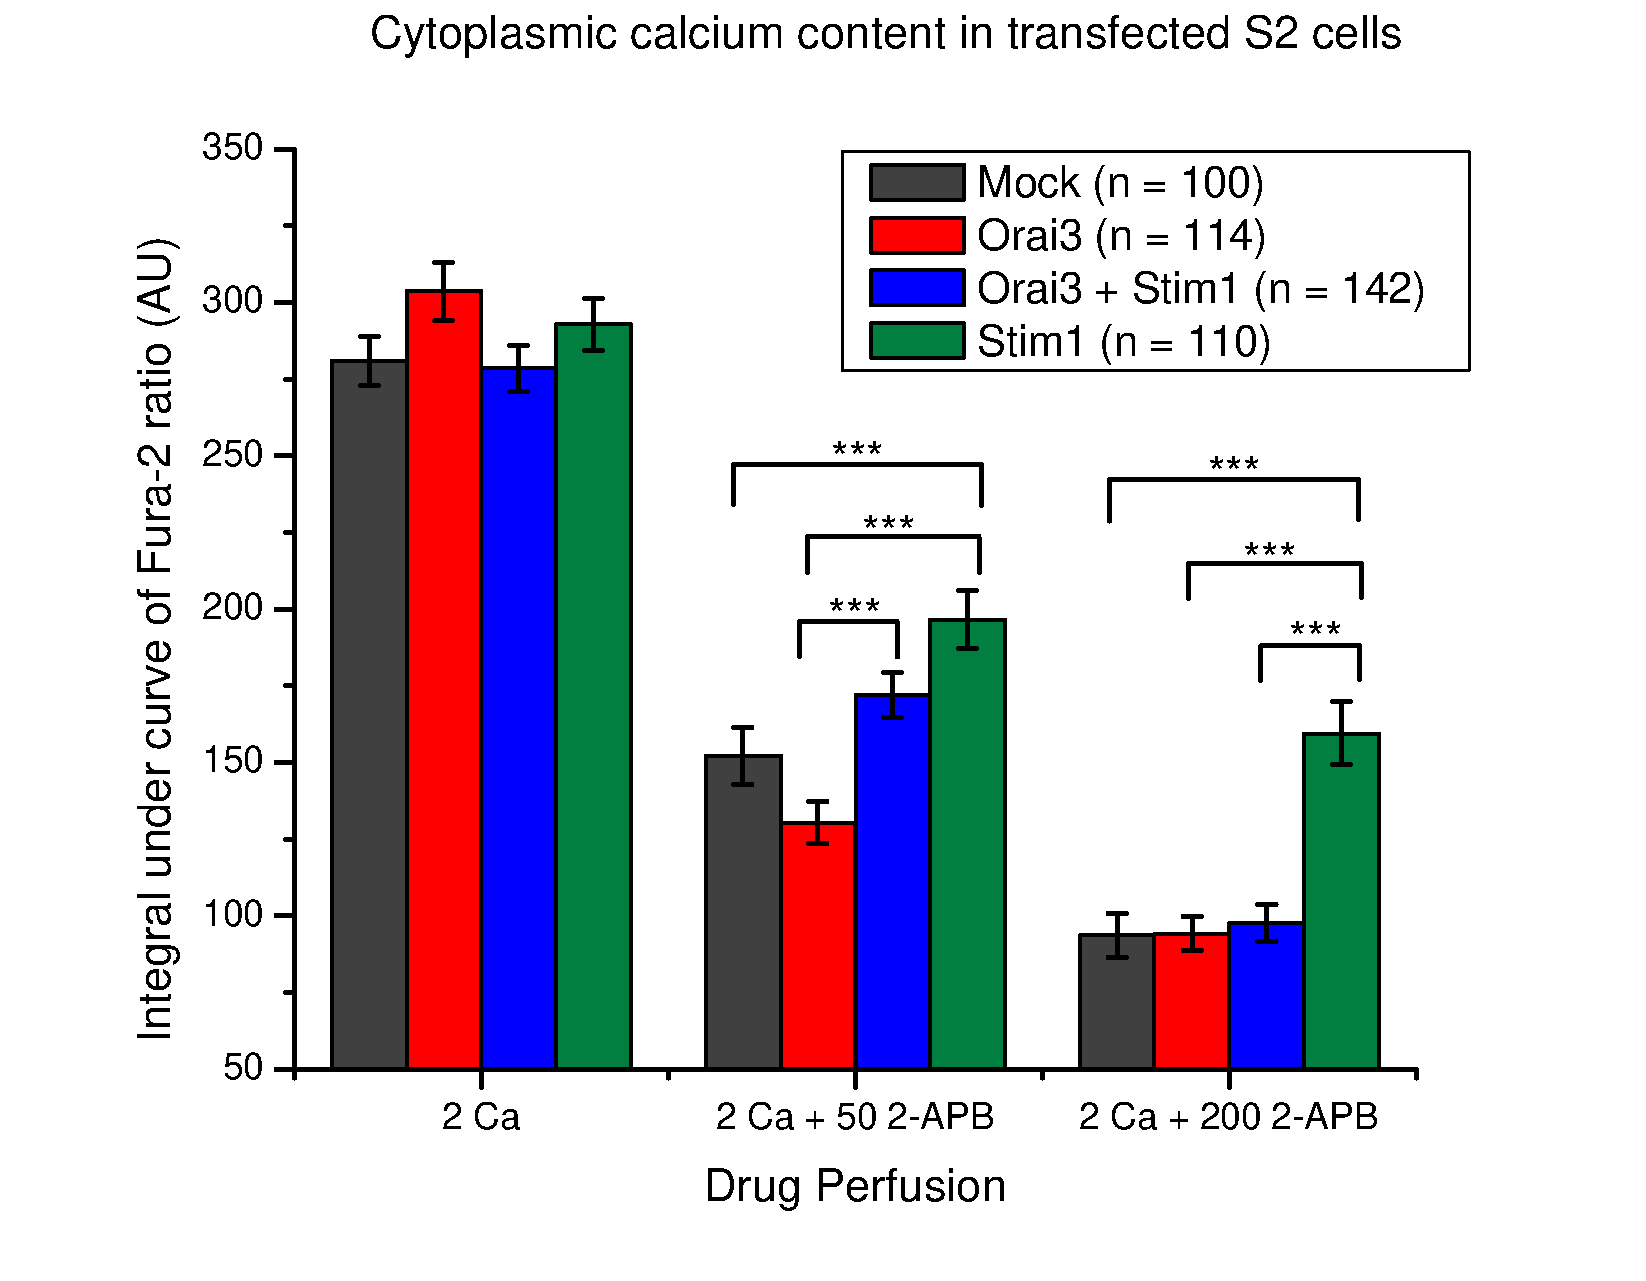
\includegraphics[clip, trim = 0 0 25mm 20mm, scale=0.6]{Figures/s2_drug_bar}
\caption[Cytoplasmic \Ca{} content in transfected S2 cells]{{\bfseries Cytoplasmic \Ca{} content in transfected S2 cells}. 
The bars represent area under the curve analysis for segments where {\bfseries 2 Ca}, {\bfseries 2 Ca + 50 $\mu$M 2-APB}, or {\bfseries 2 Ca + 200 $\mu$M 2-APB} were used to perfuse transfected S2 cells. The transfection groups are indicated in the legend. Significant differences between the transfected groups at the 0.05 significance level are indicated by ***. No significant difference was found between the 2 Ca perfusion group. Significant differences were found between the 2 Ca + 50 $\mu$M 2-APB and 2 Ca + 200 $\mu$M 2-APB perfusion groups.}
\label{fig:s2_2apb_bar}
\end{center}
\end{figure}

Figure~\ref{fig:s2_2apb_bar} displays the results of area under the curve (AUC) analysis on the three phases of treatment after store-depletion. By doing AUC analysis, the ratios generated by Fura-2 recordings were translated into cytosolic \Ca{} content of arbitrary units. The three groups in the bar graph correspond to perfusion with 2 Ca, 2 Ca + 50 $\mu$M 2-APB, and 2 Ca + 200 $\mu$M 2-APB. The perfusion time for each group was 4 minutes. A one way ANOVA was used to determine if there were significant differences in the experimental groups. If significant differences were found, Tukey's \underline{studentized} range test, was used to determine where significant differences lie between the transfection groups.  

The 2 Ca group represents an untreated period of SOCE in the transfection groups. Statistical analysis showed no significant change in cytosolic \Ca{} for this group. Functional Orai3 \Ca{} channels were expected to increase the levels of cytosolic \Ca{} during SOCE. 
%That this was not observed may be due to the \Ca{} capacity of the cell already being at maximal levels. If the S2 cell is capable of holding a finite amount of \Ca{}, and it had already reached that point, more \Ca{} channels would merely get it to that point faster, but observing further increase in \Ca{} levels would not be expected in this case.
That this was not observed may be due to the inability of Orai3 to express \emph{in the membrane}, a possibility addressed in the discussion. 

%Discussion mock:
%To determine whether the cell's cytosol was at its maximal \Ca{} carrying capacity, experiments with 2 Ca and ionomycin can be performed. After store depletion with CPA, 2 Ca can be perfusion, followed by a 2 Ca + ionomycin solution. Ionomycin is an ionophore which would raised the   \cai{} to that of the external solution. Depending on the result of perfusion with 2 Ca + ionomycin, we could say with certainty whether the maximal \Ca{} carrying capacity of the cytoplasm was reached. If for example, perfusion with ionomycin resulted in higher Ca{} levels, than was obtained without ionomycin, this would indicate that maximal levels were not obtained. 
%Discussion
%Another method for determining this would be to change the concentration of \Ca{} being used in the perfusion solution. All solutions contained 2 mM \CaCl, but decreasing the concentration to $\mu$M levels, which provide less \Ca{} for SOCE. This would result in less Ca{} being available for entry and a lower cytosolic calcium content resulting. If the \Ca{} from SOCE was still not significantly different between the transfection groups, this would allow us to conclude that the Orai3 channels were not activated solely as a function of store-depletion.


The 2 Ca + 50 2-APB experiments did show significant differences in this treatment group. 
Significant differences existed between Orai3+\stim{}-transfected cells and the Orai3 only transfected group. There were also significant differences between \stim{} only transfected cells and Orai3 only transfected cells. For both of the groups described above, the Orai3 only group showed much less cytosolic \Ca, which was unexpected. 
A significant difference was also found between mock-transfected and \stim{}-transfected cells, with the \stim{}-transfected group having higher levels of cytosolic calcium than the mock-transfected group.
The significant differences for all of the above was p $<$ 0.0001 at the 0.05 significance level. 

%Discussion:
%When only Orai3 was transfected into S2 cells and perfused with 2 Ca + 50 2-APB, a slight decrease was observed compared to mock-transfected cells, though this was not found to be significant. There were significant differences between Orai3 only and two other transfected groups: Orai3 + \stim{} and \stim{} only. That there was \emph{less} \Ca{} available in Orai3 only transfected cells, suggests that the effect of 2-APB on these  was inhibitory.
%This is supported by the finding that only \stim{}-transfected cells had significantly higher cytosolic \Ca{} than the mock-transfected cells. The difference between Orai3+\stim{} and Orai3 only transfected cells, is likely the result of the action of heterologously expressed \stim{} in this DES.


The 2 Ca + 200 2-APB showed a small but significant difference only between the \stim{}-transfected  cells and all the other groups. Again, an unexpected result which is discussed further below.  


%The \stim{} + 2-APB interaction is enhanced in higher concentrations of 2-APB. The overexpression of \stim{} in this DES may be resulting in opening of another channel by heterologous \stim{}, or alternatively slowing the deactivation of the \dorai{} responsible for the SOCE. We can see if this effect of \stim{} is specific to SOCE, by performing a similar experiment, but omitting the store depletion portion. In the absence of store-depletion, there should be no activity by \dorai{} thus any \Ca{} entry observed would likely be due to another channel. We could also test using inhibitors known to affect \dorai, such as (Ln3+?)(CITE) to determine whether the \dorai{} is being activated by \stim{} here, because \stim{} somehow changes some the characteristics of the channel. e.g. if heterologously expressed \stim{} is in the membrane, and 2-APB activates it without the need for heterologous ER \stim{} to act.

%************************

%note that perfusion of s2 cells results in near instantaneous changes in ca recordings. 
%each segment is 4 minutes long. 
%mention tukey's stat analysis
%look at probenecid - hammer that home. want to use probenecid.
%in discussion, stim1 possibilities. this vs. that.  
%Maybe Orai3 in S2s will activate in absence of store depletion.




% -eof-
